\documentclass{amsart}
\usepackage[margin=3cm]{geometry}


\usepackage{amssymb}
\usepackage[mathcal]{euscript}
\usepackage{relsize}
\usepackage{tikz}
\usepackage{tikz-cd}
% for a goodlooking table of contents
\let\oldtocsection=\tocsection 
\let\oldtocsubsection=\tocsubsection 
\renewcommand{\tocsection}[2]{\hspace{0mm}\oldtocsection{#1}{#2}}
\renewcommand{\tocsubsection}[2]{\hspace{1em}\oldtocsubsection{#1}{#2}}


\usepackage{hyperref}
\hypersetup{
    colorlinks,
    citecolor=black,
    filecolor=black,
    linkcolor=black,
    urlcolor=black
}


\usepackage{comment}
%

%symbols
\DeclareFontFamily{OT1}{pzc}{}
\DeclareFontShape{OT1}{pzc}{m}{it}{<-> s * [1.100] pzcmi7t}{}
\DeclareMathAlphabet{\mathpzc}{OT1}{pzc}{m}{it}


%for bold headers
   \usepackage{etoolbox}
    \patchcmd{\section}{\scshape}{\large\bfseries}{}{}
    \makeatletter
    \renewcommand{\@secnumfont}{\bfseries}
    \makeatother



%tikz with options
\usepackage{tikz-cd}
% \tikzcdset{arrow style=math font}
% \tikzcdset{scale cd/.style={every label/.append style={scale=#1},
%     cells={nodes={scale=#1}}}}


%bibliography
\usepackage{biblatex}
\usepackage{booktabs}
\bibliography{references}
%---------------------------------






%-------------------




\numberwithin{equation}{section}
\newtheorem{theorem}{Theorem}[section]
\newtheorem*{theorem*}{Theorem}
\newtheorem{corollary}[theorem]{Corollary}
\newtheorem{lemma}[theorem]{Lemma}
\newtheorem{proposition}[theorem]{Proposition}
\theoremstyle{definition}
\newtheorem{question}{Question}
\newtheorem{problem}{Problem}
\newtheorem{definition}[theorem]{Definition}
\newtheorem{remark}[theorem]{Remark}
\newtheorem{example}[theorem]{Example}


\def\Grp{\mathsf{Grp}}
\def\Cov{\mathsf{Cov}}
\def\Subgroup{\mathsf{Subgroup\;}}
\def\Arr{\mathsf{Arr}}
\def\Obj{\mathsf{Obj}}
\def\Set{\mathsf{Set}}
\def\CC{\mathsf{C}}
\def\Cat{\mathsf{Cat}}
\def\Gpd{\mathsf{Gpd}}
\def\Set{\mathsf{Set}}
\def\Hom{\mathsf{Hom}}
\def\ZZ{\mathbb{Z}}
\def\RR{\mathbb{R}}
\def\id{\mathsf{id}}
\def\Id{\mathsf{Id}}

\newcommand{\F}{\mathcal{F}}
\newcommand{\cc}{\mathcal{C}}
\newcommand{\qq}{\mathcal{Q}}
\newcommand{\ee}{\mathcal{E}}
\newcommand{\bb}{\mathcal{B}}
\newcommand{\Eps}{\mathcal{E}}
\newcommand{\dd}{\mathcal{D}}
\newcommand{\Aut}{\mathrm{Aut}}
\newcommand{\colim}{\mathrm{colim}}
\newcommand{\dom}{\mathrm{dom}}
\newcommand{\cod}{\mathrm{cod}}

\newcommand{\Tau}{\mathcal{T}}
\newcommand{\Crossed}{\textsf{Crossed}}
% % \def\Crossed{\textsf{Crossed}}
% \DeclareMathOperator{\Crossed}{Crossed}
\newcommand{\loc}{\textsf{loc }}
\newcommand{\cantor}{\textsf{cantor}}
\newcommand{\Loc}{\textsf{Loc }}
\newcommand{\GOCat}{\textsf{GOCat}}
\newcommand{\Iso}{\textsf{Iso}}
\newcommand{\GOCrossed}{\textsf{GOCrossed}}
\newcommand{\Div}{\text{Div}}
\newcommand{\cDiv}{\widetilde{\text{Div}}}



% HOW TO EMBED PICTURES
% !!!!!!!!!!!!!!!!!!!!!!!!!!!
% \begin{center}\label{cablingpic}
%     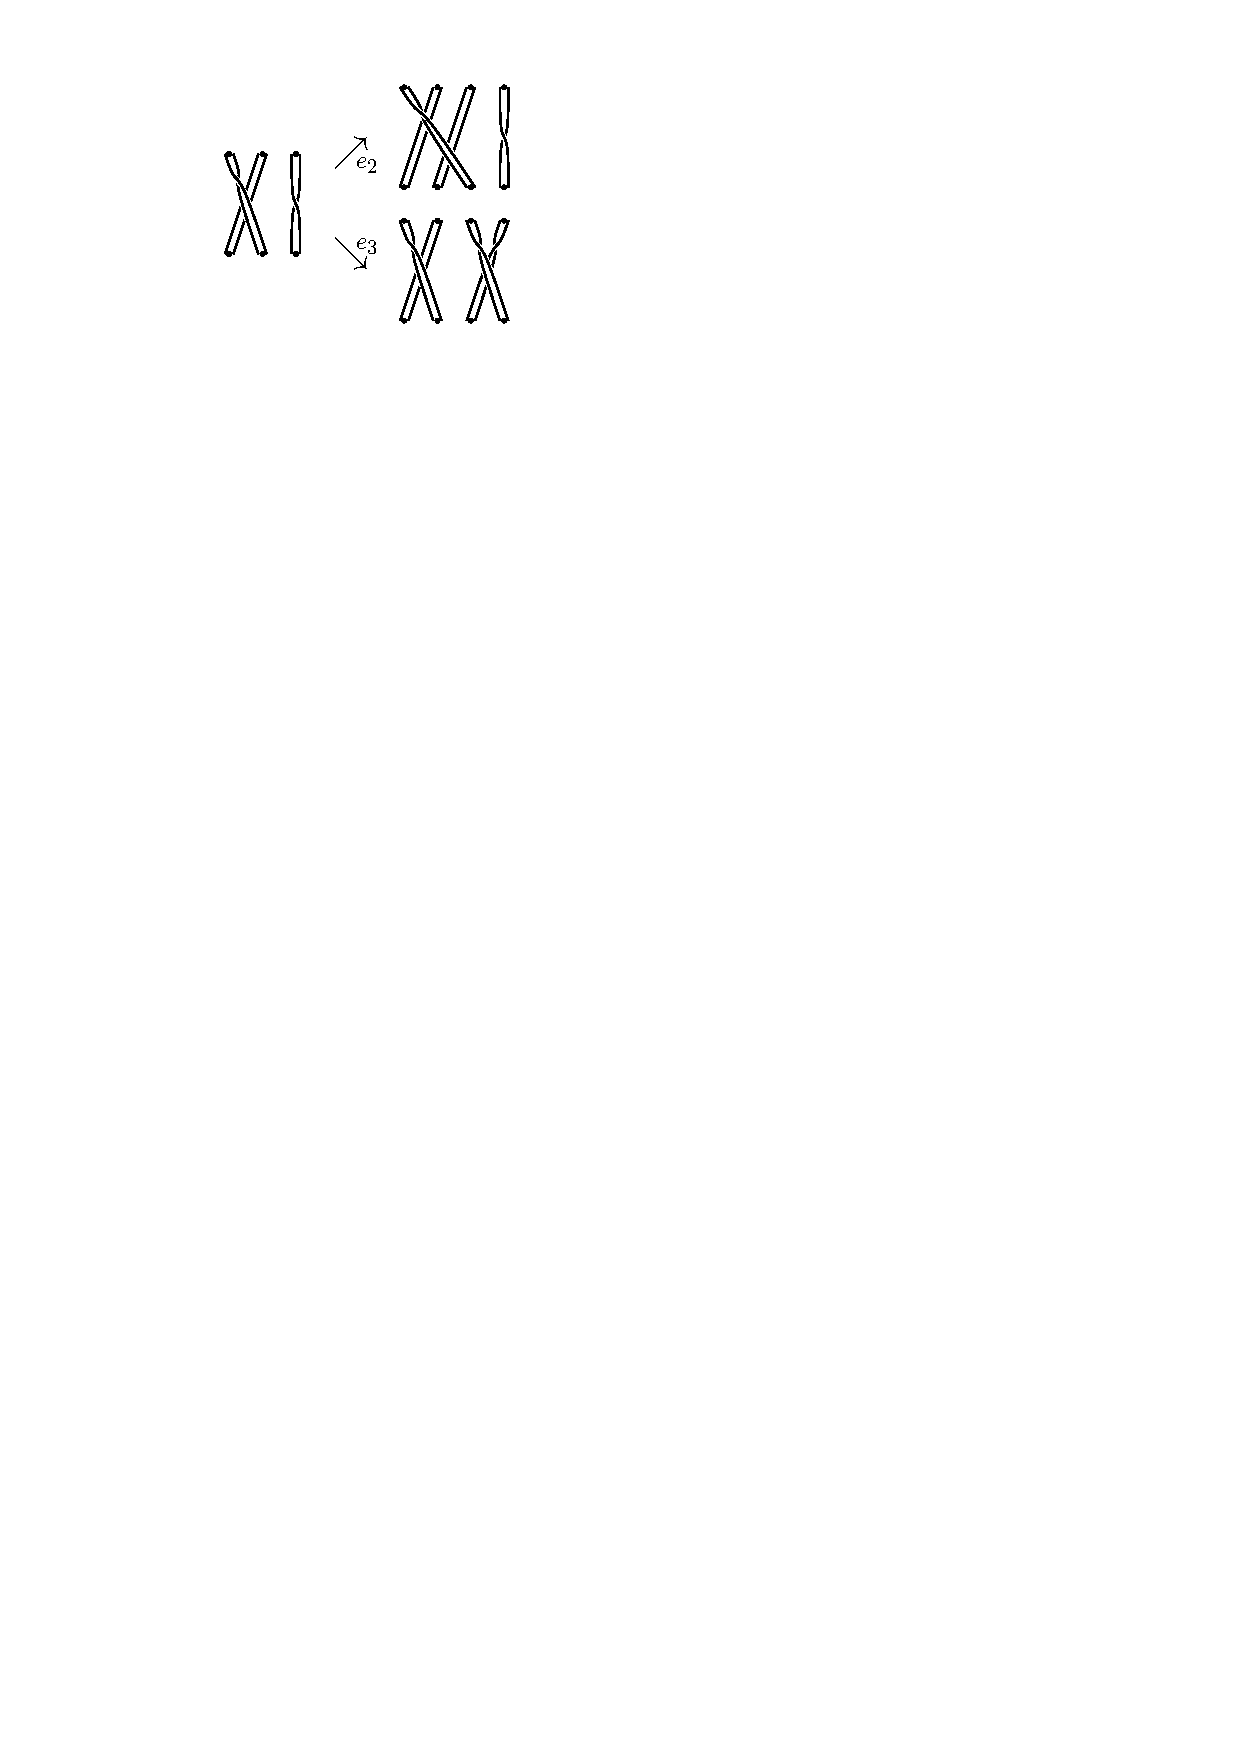
\includegraphics[scale = 1.2]{pictures/zaplet-per.pdf}
% \end{center}


% \begin{figure}[bh]
%\noindent\centering{
% \includegraphics[width=120mm]{curves.eps}             % \caption{Ступенчатая функция потерь}
% \label{figCurves}
%\end{figure}

\usepackage{quiver}
\usetikzlibrary{angles,calc,quotes,babel,arrows.meta,decorations.markings,plotmarks}


\begin{document}

\title[A categorical generalization for Thompson's groups]{A categorical generalization for Thompson's groups}


\author{A. Semidetnov}
\email{artemsemide≈tnov@gmail.com, Artem.Semidetnov@etu.unige.ch}
\address{Universit\'{e} de Gen\`{e}ve, Section de Math\'{e}matiques, Route de Drize 7, Villa Battelle, 1227 Carouge, Switzerland}


\begin{abstract}
    We propose a generalization of Thompson’s groups obtained via the notion of a crossed $\cc$-group for a small category $\cc$. This construction subsumes, as a particular instance, Zaremsky’s groups defined by cloning systems, thereby providing a unified categorical framework for such generalizations. We prove that the class of our generalized Thompson's groups is closed under taking subgroups. 
\end{abstract}

\maketitle


\tableofcontents

\section*{Introduction}
Thompson’s groups possess a remarkably rich algebraic structure, and numerous generalizations have appeared in the literature. Notable examples include those developed in \cite{aramayona2019asymptoticmappingclassgroups, belk2007thompsonsgroupf, zaremsky2022usersguidecloningsystems, Witzel_2019}. Each of these constructions employs Ore categories and their localizations as the principal framework for constructing the corresponding groups.  

In this note, we propose an additional generalization, which also makes essential use of Ore categories and their localizations. Although our approach is conceptually related to the perspectives of \cite{Witzel_2019, belk2007thompsonsgroupf}, we aim to present it from a distinct viewpoint that may clarify certain algebraic properties of these groups. For a standard treatment of the original Thompson groups \( F \), \( T \), and \( V \), we refer the reader to \cite{MR1426438}.  

To preserve the continuity of exposition, detailed computational proofs are collected at the end of the paper.

\section{Crossed groups}

\subsection{Definitions}

We adopt the convention of right-to-left composition throughout this article; that is, for morphisms $\bullet\xrightarrow{f}\bullet\xrightarrow{g}\bullet$, we denote the composition by $fg$.

For a category $\mathcal{C}$, we denote the hom-sets $\hom_{\mathcal{C}}(a,b)$ by $\mathcal{C}(a,b)$. When $\mathcal{C}$ is a small category and $\mathcal{D}$ is any category, the functors $\mathcal{C} \to \mathcal{D}$ form a category whose objects we call $\mathcal{C}$-objects in $\mathcal{D}$. This allows us to speak of $\mathcal{C}$-groups, $\mathcal{C}$-spaces, and so forth. Crossed simplicial groups were introduced by Fiedorowicz and Loday~\cite{fied_loday} and, under the name skew-simplicial groups, by Krasauskas~\cite{krasauskas_skew-simplicial_1987}. Berger and Moerdijk~\cite{Berger_2010} generalized this notion to that of a crossed $\mathcal{C}$-group, where $\mathcal{C}$ is a small category. We present two equivalent definitions of crossed $\mathcal{C}$-groups below. Since crossed $\mathcal{C}$-groups generalize $\mathcal{C}$-groups, we sometimes refer to the latter as \emph{genuine} $\mathcal{C}$-groups for emphasis.

A category $\mathcal{C}$ is called \emph{gaunt} if it has no nontrivial isomorphisms. For the remainder of this section, we fix a small, gaunt, connected category $\mathcal{C}$.

\begin{definition}
A \emph{crossed $\mathcal{C}$-group} consists of a collection of groups $\{G_c\}_{c \in \mathcal{C}}$ together with a small category $\mathcal{C}G$ satisfying:
\begin{enumerate}
    \item $\operatorname{Ob}(\mathcal{C}G) = \operatorname{Ob}(\mathcal{C})$,
    \item $\mathcal{C}$ is a subcategory of $\mathcal{C}G$,
    \item $\operatorname{Aut}_{\mathcal{C}G}(c) = G_c^{\mathrm{op}}$ for all $c \in \mathcal{C}$,
    \item Every morphism in $\mathcal{C}G$ factors uniquely as $\varphi \cdot g$, where $\varphi \in \mathcal{C}(c_1, c_2)$ and $g \in G_{c_2}$.
\end{enumerate}
The category $\mathcal{C}G$ is called the \emph{category of the crossed $\mathcal{C}$-group} $G$.
\end{definition}

We now derive an equivalent definition. Let $G$ be a crossed $\mathcal{C}$-group. For any objects $a, b \in \mathcal{C}$, morphism $f \in \mathcal{C}(a,b)$, and element $g \in G_a$, there exist unique morphisms $g^*(f) \in \mathcal{C}(a,b)$ and $f^*(g) \in G_b$ such that
\[
g \cdot f = g^*(f) \cdot f^*(g).
\]

\begin{lemma}
The assignment $f^* : G_{\operatorname{dom} f} \to G_{\operatorname{cod} f}$ defines a $\mathcal{C}$-set structure. Furthermore, if the maps $g^*$ act trivially on morphisms, then this structure is an genuine $\mathcal{C}$-group.
\end{lemma}

\begin{proof}
The proof is a straightforward computation and is omitted.
\end{proof}

This lemma motivates the following equivalent definition, which more closely resembles that of~\cite{Berger_2010}.

\begin{definition}\label{def_berger}
A \emph{crossed $\mathcal{C}$-group} is a functor $G : \mathcal{C}^{\mathrm{op}} \to \mathsf{Set}$ equipped with:
\begin{enumerate}
    \item A group structure on $G_c$ for each $c \in \mathcal{C}$,
    \item A left $G_c$-action on $\mathcal{C}(c, s)$ for every $s \in \mathcal{C}$,
\end{enumerate}
satisfying the following axioms for all composable morphisms and group elements:
\begin{enumerate}
    \item $g^*(fh) = g^*(f) \cdot (f^*(g))^*(h)$,
    \item $g^*(\operatorname{id}_c) = \operatorname{id}_c$,
    \item $f^*(hg) = (g^*(f))^*(h) \cdot f^*(g)$,
    \item $f^*(1_{\operatorname{dom} f}) = 1_{\operatorname{cod} f}$.
\end{enumerate}
\end{definition}

A morphism between crossed $\mathcal{C}$-groups $G_*$ and $H_*$ is a functor $\mathcal{C}G \to \mathcal{C}H$ that is the identity on the subcategory $\mathcal{C}$. This defines the category $\mathsf{Crossed}(\mathcal{C})$ of crossed $\mathcal{C}$-groups. The following lemma is useful. 



\begin{lemma}\label{algebraic-properties}
    The category $\Crossed(\cc)$ of crossed $\cc$-groups 
    \begin{enumerate}
        \item is closed under pullbacks of monomorphisms;
        \item has a zero object (i.e. an object which is both initial and terminal).
    \end{enumerate}
\end{lemma}

% \begin{definition}
%     Let $\Crossed$ be the category with 
%     \begin{enumerate}
%         \item Objects being pairs $(\cc, G)$, where $\cc \in \Cat$ and $G \in \Crossed(\cc)$
%         \item A morphism $(\cc, G) \to (\dd, H)$ is given by a functor $f \colon \cc G \to \dd H$ such that $f(\cc) \subset \dd$. 
%     \end{enumerate}
% \end{definition}
\subsection{Examples}

We now introduce our main example of a small gaunt category $\mathcal{T}$, which will be used to construct the standard Thompson's groups $F$, $T$, and $V$.

\begin{definition}
The category $\mathcal{T}$ is defined by the following presentation:
\begin{enumerate}
    \item The objects are natural numbers $1, 2, \dots$,
    \item For each $n$, there are $n$ morphisms $\mathcal{T}(n, n+1)$, denoted $e_1^{(n)}, \dots, e_n^{(n)}$ (Superscripts will often be omitted),
    \item These morphisms satisfy the relations:
    \[
    e_j e_i = e_i e_{j+1}, \quad \text{for } i < j.
    \]
\end{enumerate}
\end{definition}

\begin{remark}
The category $\mathcal{T}$ admits a combinatorial description: morphisms $\mathcal{T}(n, m)$ correspond bijectively to ordered $n$-tuples of rooted binary trees with a total of $m$ leaves. Composition $\mathcal{T}(n, m) \times \mathcal{T}(m, k) \to \mathcal{T}(n, k)$ corresponds to concatenation of trees.
\end{remark}

\begin{remark}
The given relations resemble the standard simplicial identities. Indeed, if we added the relations $e_i e_i = e_i e_{i+1}$, the resulting category would be equivalent to $\Delta_{\mathrm{inj}}$.
\end{remark}
% \subsection{Examples.} Here we introduce our main example of a small gaunt category $\Tau$. This category will be later used to produce the standard Thompson's groups $F, T, V$. 
% % Here we introduce the main example of a 


% \begin{definition}
%     We define the category $\Tau$ by the following presentation.
%     \begin{enumerate}
%         \item The objects of the category $\Tau$ are the natural numbers $1, 2, \ldots$.
%         \item For each $n$, there are $n$ morphisms $\Tau(n, n+1)$, which we denote by $e^{(n)}_1, \ldots, e^{(n)}_n$. Hereafter, the superscripts will often be omitted.
%         \item These morphisms are subject to the following relations:
%         $$e_j e_i = e_i e_{j+1}, \quad i < j.$$
%     \end{enumerate}
% \end{definition}

% \begin{remark}
%     The category $\Tau$ has the following combinatorial description: the morphisms $\Tau(n, m)$ are in bijection with ordered sets of $n$ rooted binary trees with a total of $m$ leaves. The composition $\Tau(n, m) \times \Tau(m, k) \to \Tau(n, k)$ corresponds to the concatenation of trees.
% \end{remark}

% \begin{remark}\label{tau-simplicial}
%     One may find the standard simplicial identities in resemblance with the ones above. In fact, if we add the relations $e_ie_i = e_ie_{i+1}$ to it this category would be seen to be equivalent to the category $\Delta_{\text{inj}}$. 
% \end{remark}

The figure below depicts morphisms $1 \to 4$ (top left) and $4 \to 7$ (bottom left). Their composition---the morphism $1 \to 7$---is shown on the right.

\begin{figure}[h]
\centering
\begin{tikzpicture}[line width=0.8pt, scale=0.44]
  \draw
   (-3,-3) -- (0,0) -- (3,-3)   (1,-3) -- (-1,-1)   (-1,-3) -- (0,-2);
  \filldraw
    (-3,-3) circle (1.5pt)   (0,0) circle (1.5pt)   (3,-3) circle (1.5pt)   (-1,-1) circle (1.5pt)  (-1,-3) circle (1.5pt)   (0,-2) circle (1.5pt)   (1,-3) circle (1.5pt);   %(2,0) circle (1.5pt)  (4,0) circle (1.5pt)   (6,0) circle (1.5pt);

  \begin{scope}[yshift=-5cm]
   \draw
    (-4,-1) -- (-3,0) -- (-2,-1)   (1,-2) -- (3,0) -- (5,-2)   (3,-2) -- (2,-1);
   \filldraw
    (-4,-1) circle (1.5pt)   (-3,0) circle (1.5pt)   (-2,-1) circle (1.5pt)   (-1,0) circle (1.5pt)   (1,0) circle (1.5pt)   (1,-2) circle (1.5pt)   (3,0) circle (1.5pt)   (5,-2) circle (1.5pt)   (3,-2) circle (1.5pt)   (2,-1) circle (1.5pt);   %(5,0) circle (1.5pt);
    \node at (10,2) {$=$};
  \end{scope}
   
  \begin{scope}[xshift=16cm]
   \draw
    (-3,-3) -- (0,0) -- (3,-3)   (1,-3) -- (-1,-1)   (-1,-3) -- (0,-2)
    (-4,-4) -- (-3,-3) -- (-2,-4)   (1,-5) -- (3,-3) -- (5,-5)   (3,-5) -- (2,-4);
   \filldraw
   (-3,-3) circle (1.5pt)   (0,0) circle (1.5pt)   (3,-3) circle (1.5pt)
   (-1,-1) circle (1.5pt)   (-1,-3) circle (1.5pt)   (0,-2) circle (1.5pt)
   (1,-3) circle (1.5pt)      
     (-4,-4) circle (1.5pt)   (-2,-4) circle (1.5pt)  (1,-5) circle (1.5pt)   (5,-5) circle (1.5pt)   (3,-5) circle (1.5pt);
  \end{scope}
\end{tikzpicture}
\end{figure}


% Often, we will be interested in its slice category $\Tau_0 := 1/\Tau$. From the tree-based description above, it is clear that the objects of $\Tau_0$ are all possible rooted binary trees. It is also evident that, as a category, $\Tau_0$ is thin (i.e., it is a preorder). Alternatively, the inclusion of trees as rooted subtrees of one another defines the entire categorical structure of $\Tau_0$. Let $f \colon 1 \to n$ be an element of the slice category $\Tau_0$; then, the multiplication of $f$ by $e_i \colon n \to n+1$ will be called \textit{caret addition}. The subtree added to $f$ in this process will be called a caret. In the figure below, we see how a red caret is added to the tree $1 \to 3$ (black), resulting in the tree $1 \to 4$.


We will often work with the slice category $\mathcal{T}_0 := 1/\mathcal{T}$. From the tree description, the objects of $\mathcal{T}_0$ are all rooted binary trees, and $\mathcal{T}_0$ is thin (i.e., a preorder). Alternatively, the categorical structure of $\mathcal{T}_0$ is determined by the inclusion of trees as rooted subtrees.

Let $f \colon 1 \to n$ be an object of $\mathcal{T}_0$. Multiplication of $f$ by $e_i \colon n \to n+1$ is called \emph{caret addition}. The subtree added to $f$ in this process is called a \emph{caret}. The figure below shows a red caret added to the tree $1 \to 3$ (black), resulting in the tree $1 \to 4$.

Every morphism in $\mathcal{T}_0$ can be expressed as a composition of caret additions.

\begin{center}
    \begin{tikzpicture}[
  level distance=1.2cm,
  sibling distance=3cm,
  every node/.style={circle, draw, fill=black, inner sep=1.5pt},
  level 2/.style={sibling distance=1.5cm}
]

\node {}
  child {node {}
    child {node {}}
    child {node {}
      child [edge from parent/.style={draw=red, thick}] {node[fill=red] {}}
      child [edge from parent/.style={draw=red, thick}] {node[fill=red] {}}
    }
  }
  child {node {}};

\end{tikzpicture}
\end{center}
% It is evident that each morphism in $\Tau_0$ can be written as a composition of caret additions.

\subsection*{Crossed $\Tau$-groups}

% If one unfolds the definition of the crossed $\cc$ group in the case of $\cc = \Tau$, one sees that to define a crossed $\Tau$ group amounts to defining a sequence of groups $G_n$ for $n = 1, 2, \ldots$ and functions $e_i : G_n \to G_{n+1}$ such that they satisfy certain relations.

Specializing to the case $\mathcal{C} = \mathcal{T}$, we find that a crossed $\mathcal{T}$-group is specified by a sequence of groups $\{G_n\}_{n \geq 1}$ together with maps
\[
e_i : G_n \longrightarrow G_{n+1}, \quad \text{for } i = 1, \ldots, n,
\]
satisfying certain relations.

Since every morphism in $\mathcal{T}G$ can be uniquely written as $t \cdot g$ with $t \in \mathcal{T}$ and $g \in G_*$, one may visualize such a morphism as the tree diagram representing $t$ decorated by the group element $g$. This provides a useful intuition, though it is not a formal definition.

We now present several examples of crossed $\mathcal{T}$-groups. It will be explained in Lemma \ref{Crossed-Tau} that these are indeed crossed $\Tau$ groups. 


\subsubsection{The braided crossed $\Tau$-group}

This example, while not the simplest, is particularly instructive for our purposes.

Let $B_n$ denote the Artin braid group on $n$ strands. For each $n$, there are $n$ \emph{cabling maps}
\[
e_i : B_n \to B_{n+1}, \quad i = 1, \ldots, n.
\]
The map $e_i$ replaces the $i$-th strand with two parallel strands. These maps define the crossed $\mathcal{T}$-group $B_*$ and its associated category $\mathcal{T}B_*$.


\begin{figure}[htbp]
\noindent\centering{
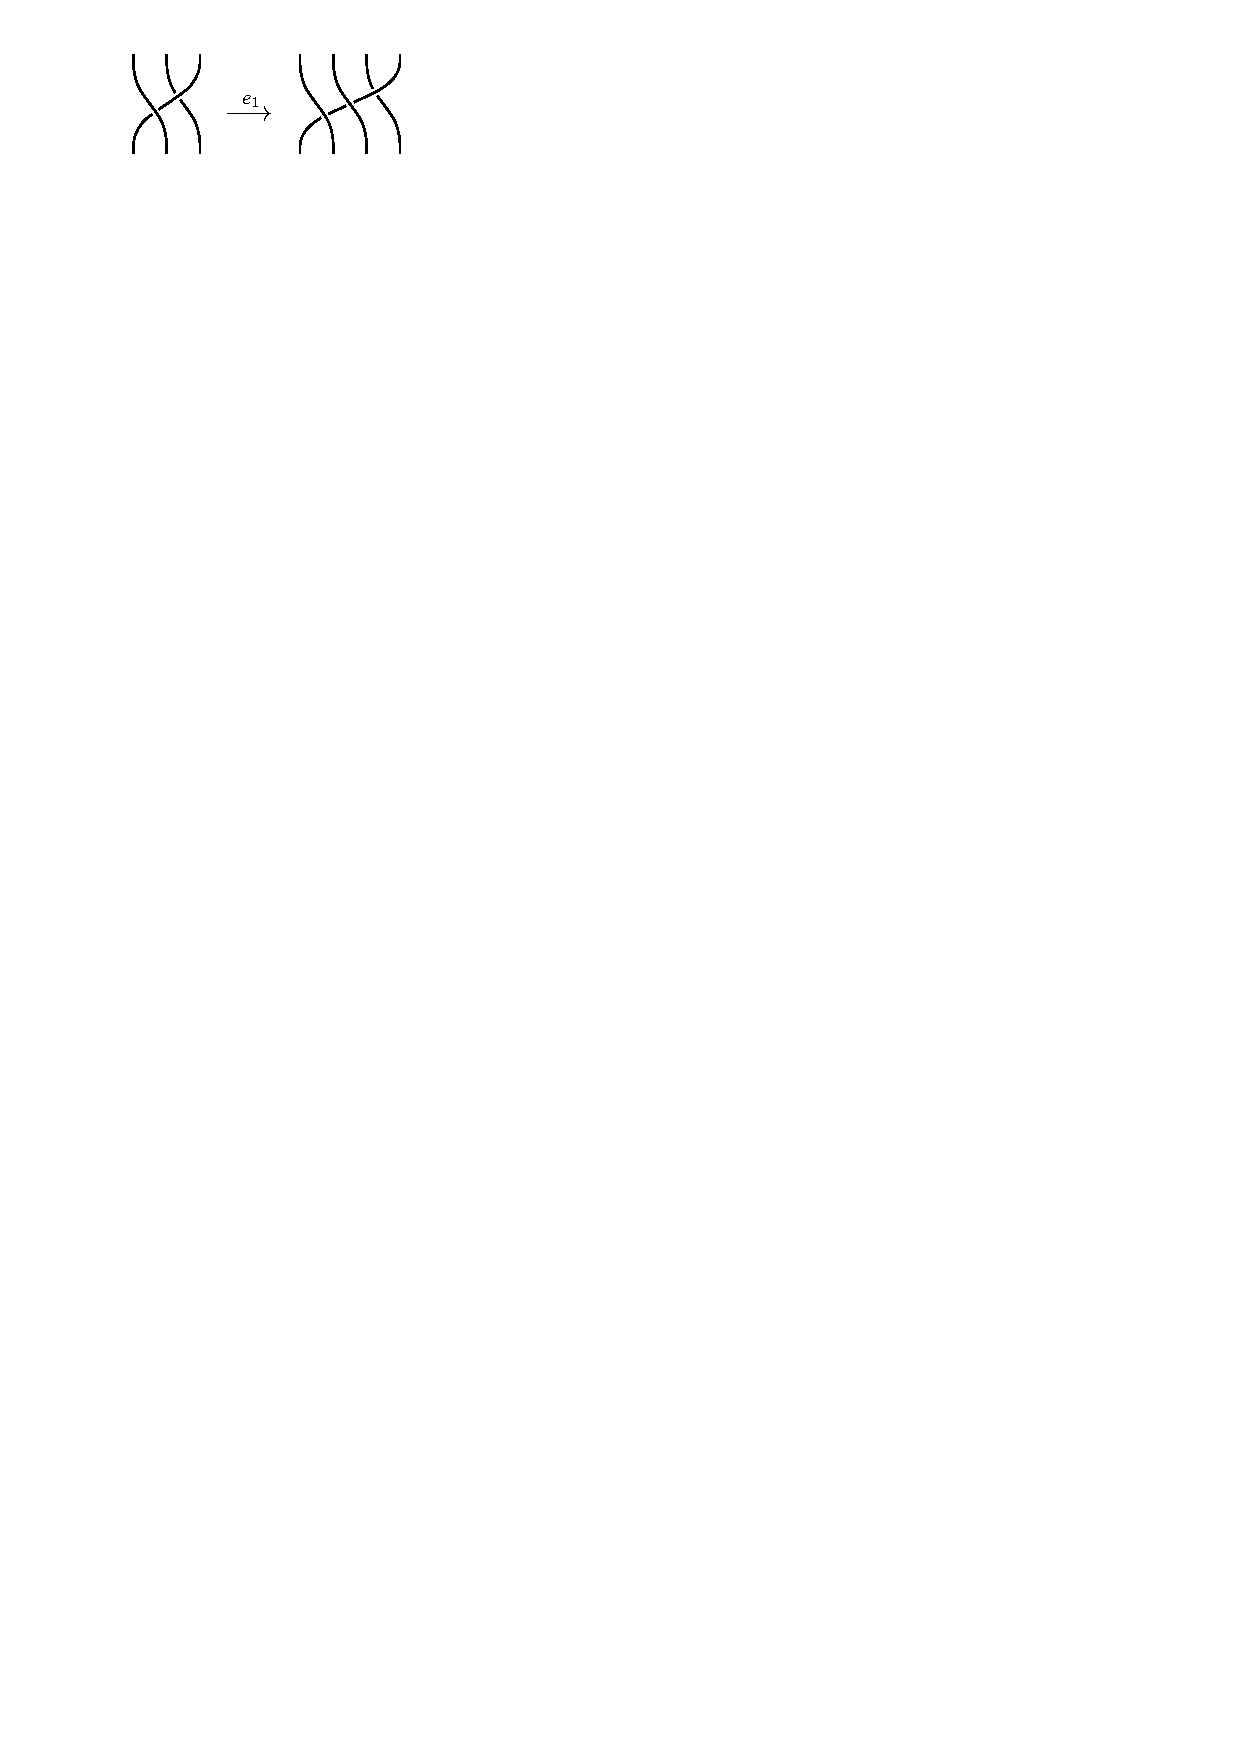
\includegraphics[width=60mm]{pictures/cabling.pdf}
\caption{Example of the cabling operation}
\label{cabling}}
\end{figure}


\begin{figure}[htbp]
\noindent\centering{
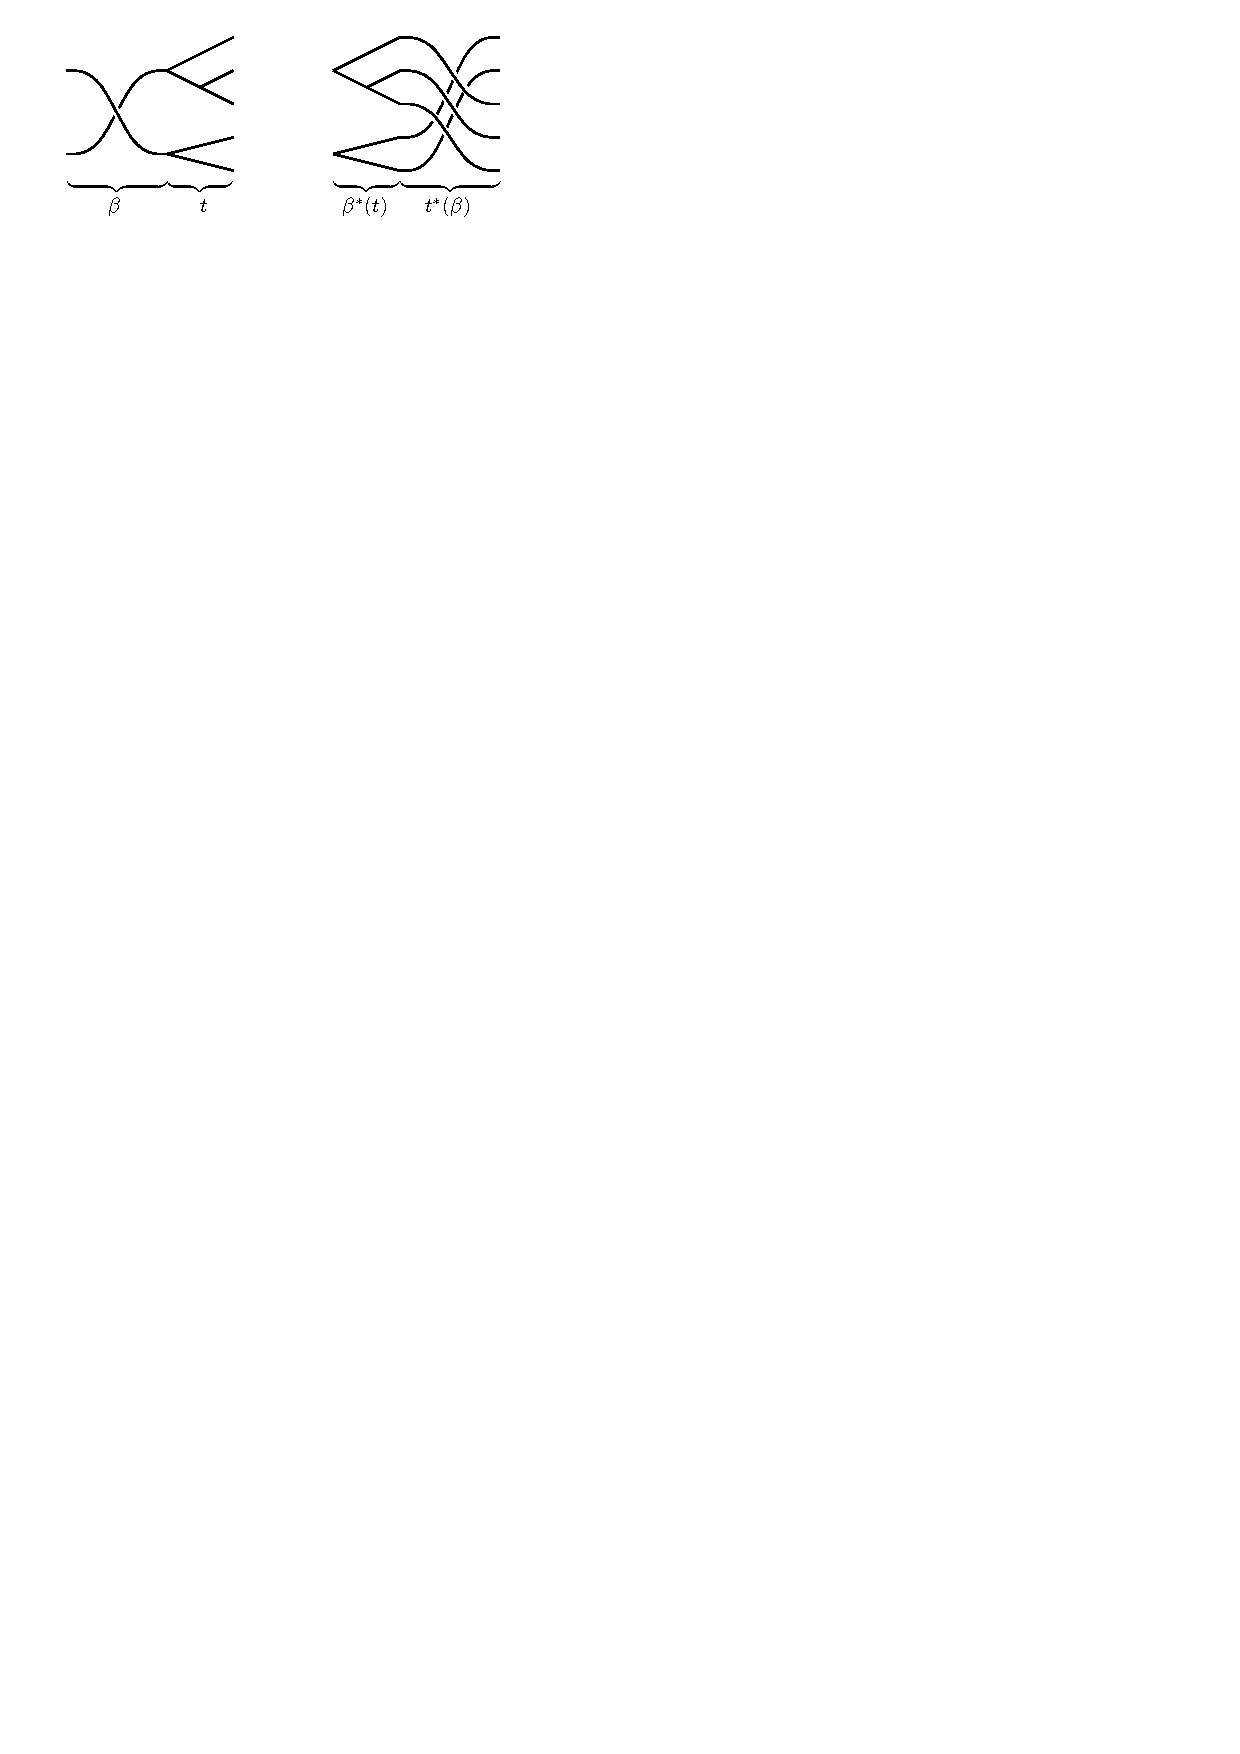
\includegraphics[width=100mm]{pictures/action_eg.pdf}
\caption{Example of a morphism $2 \to 5$ structure maps in $\Tau B$}
\label{actionOrigin}}
\end{figure}

\subsubsection{The hyperoctahedral crossed $\Tau$-group}
% We now describe a specific crossed $\Tau$-group $H_*$. For each $n \ge 1$, let $(\ZZ/2)^n \rtimes S_n$, where $S_n$ acts on $(\ZZ/2)^n$ by permuting coordinates. This group is commonly referred to as the \emph{octahedral group} or, in a combinatorial context, as the \emph{group of $n$ cards}. Next, we define a family of maps 
% \(
% e_i \colon H_n \longrightarrow H_{n+1}, \quad 1 \le i \le n,
% \) 
% given by

% Put $$e_i(\underbrace{(\varepsilon_1, \ldots, \varepsilon_n)}_{\in (\ZZ/2)^n}, \sigma) = ((\varepsilon_1, \ldots, \varepsilon_i, \varepsilon_i, \ldots, \varepsilon_n), e_i^{\varepsilon_i}(\sigma))$$
% where
% \begin{itemize}
%     \item $e_i^0(\sigma)$ denotes the standard cabling operation for permutations, analogous to the usual cabling in the braid group, and
%     \item $e_i^1(\sigma)$ denotes the \emph{twisted cabling}, in which the $i$-th strand is replaced by two intersecting strands, as illustrated in Figure~\ref{cablingpic}.
% \end{itemize}

We now describe a specific crossed $\mathcal{T}$-group $H_*$. For each $n \geq 1$, define
\[
H_n = (\mathbb{Z}/2)^n \rtimes S_n,
\]
where $S_n$ acts on $(\mathbb{Z}/2)^n$ by permuting coordinates. This group is commonly called the \emph{hyperoctahedral group} or, in combinatorial contexts, the \emph{group of signed permutations}.

We define maps $e_i \colon H_n \longrightarrow H_{n+1}$ for $1 \leq i \leq n$ by:
\[
e_i((\varepsilon_1, \ldots, \varepsilon_n), \sigma) = ((\varepsilon_1, \ldots, \varepsilon_i, \varepsilon_i, \ldots, \varepsilon_n), e_i^{\varepsilon_i}(\sigma)),
\]
where:
\begin{itemize}
    \item $e_i^0(\sigma)$ denotes the standard cabling operation for permutations, analogous to the braid group cabling,
    \item $e_i^1(\sigma)$ denotes \emph{twisted cabling}, where the $i$-th strand is replaced by two intersecting strands, as illustrated in Figure~\ref{cablingpic}.
\end{itemize}


% \begin{remark}
%     One can visualize elements of $H_n$ as $n$ twisted $\pmod 2$ permuted strands. In this description, the maps $e_i$ take the following form. 
%     \begin{center}\label{cablingpic}
%     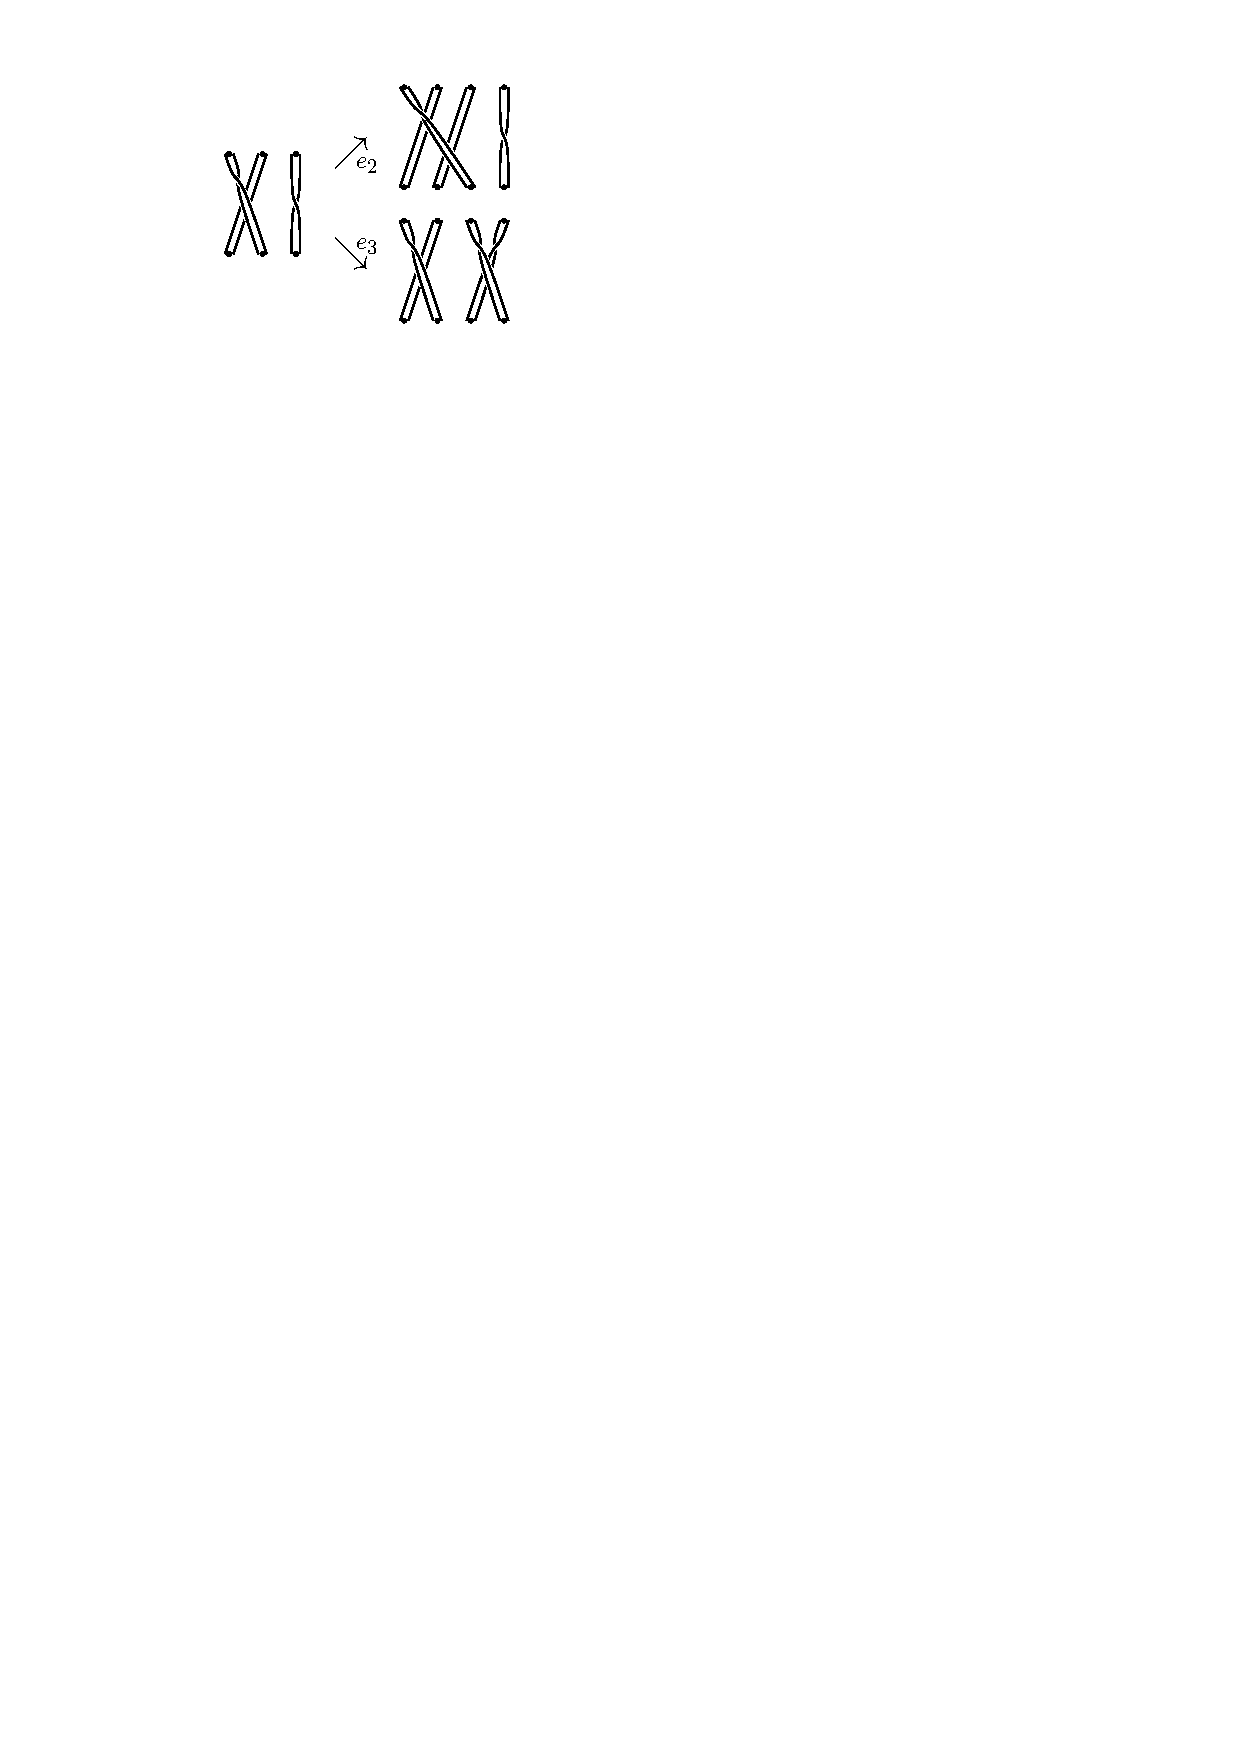
\includegraphics[scale = 1.2]{pictures/zaplet-per.pdf}
% \end{center}
% \end{remark}

\begin{remark}
Elements of $H_n$ can be visualized as $n$ strands with mod~2 twists, permuted according to $\sigma$. The maps $e_i$ then correspond to inserting either parallel or intersecting strands at position $i$.
\begin{center}\label{cablingpic}
    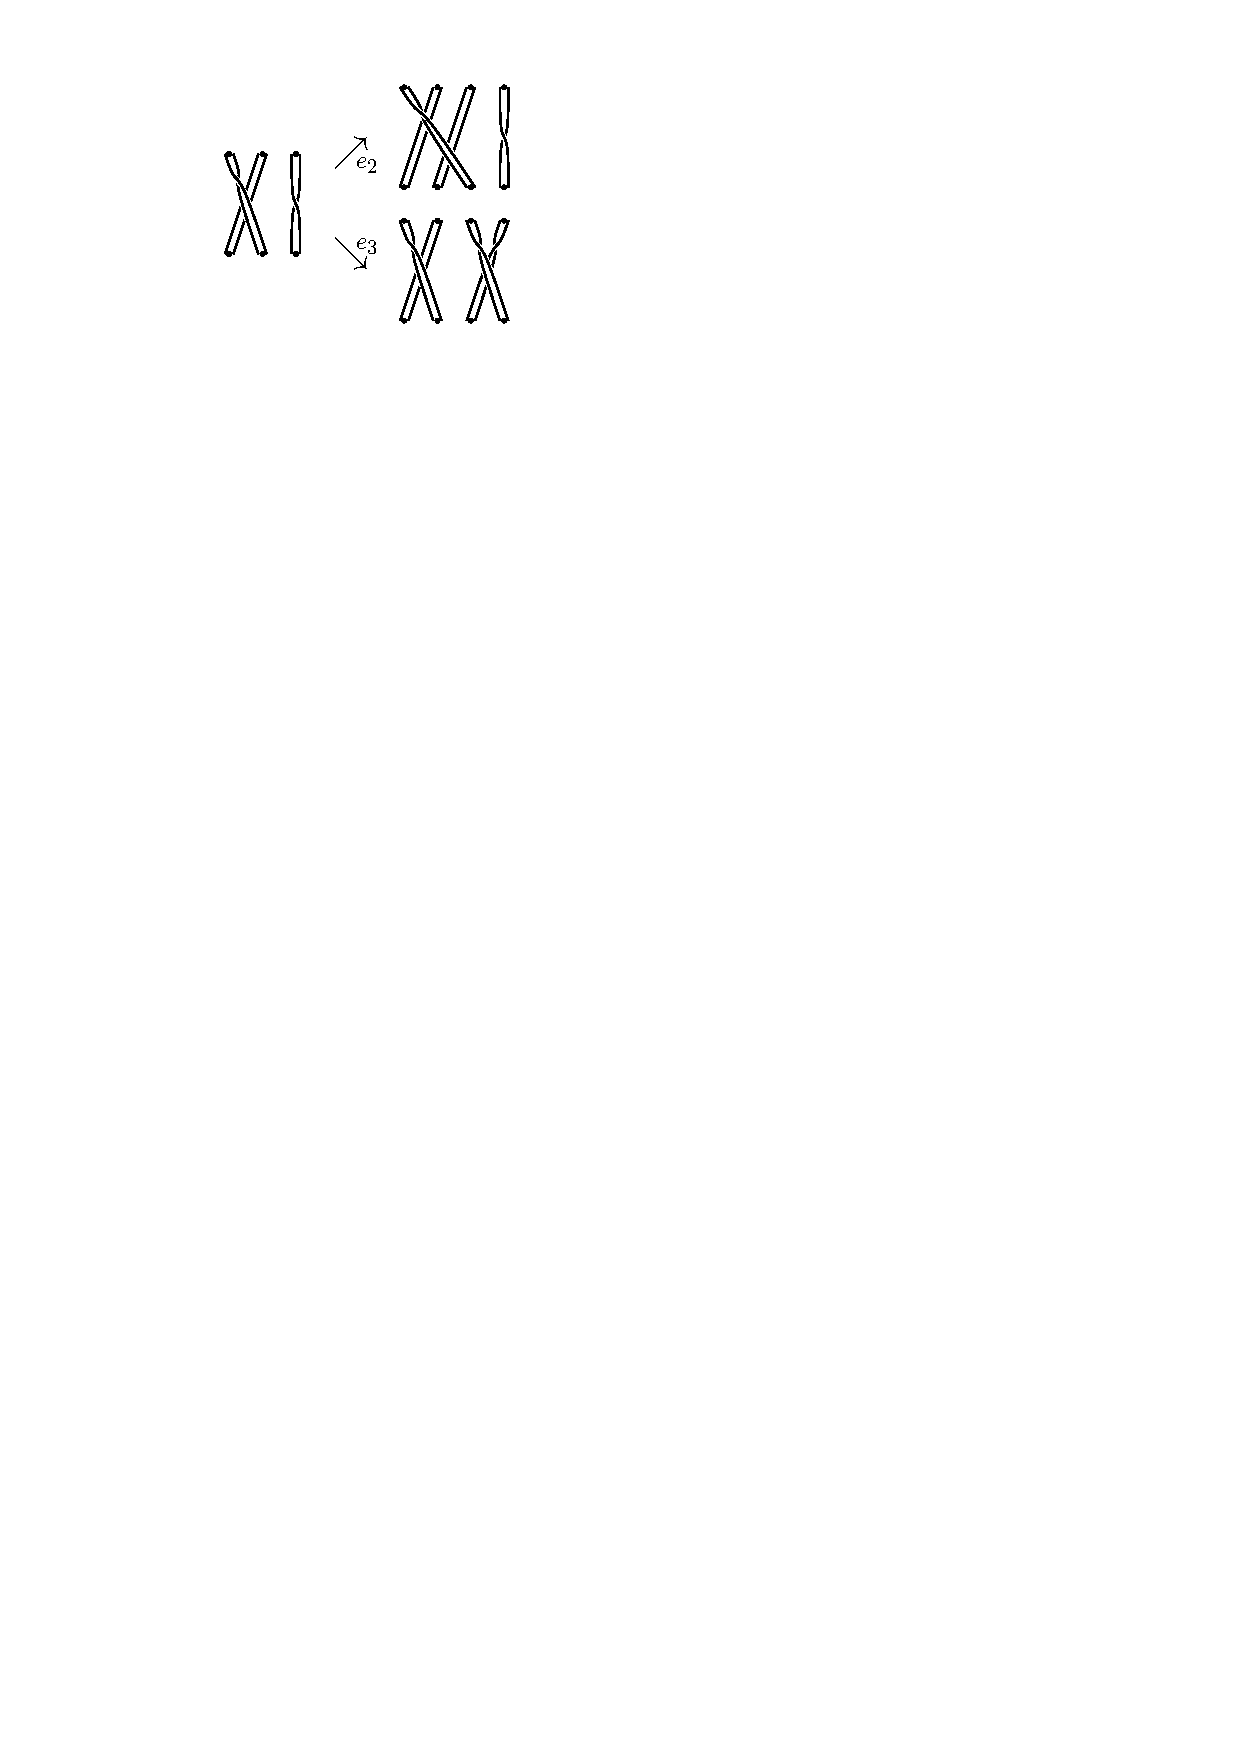
\includegraphics[scale = 1.2]{pictures/zaplet-per.pdf}
\end{center}
\end{remark}


% \subsubsection{The ribbon braid group example}
% This example is a mix of the two examples above. Introduce the ribbon braid group $RB_n$. 

% \subsubsection{Examples of subgroups of $H_*$}
% Here we describe 7 crossed $\Tau$-subgroups of $H_*$. 

% \begin{definition}
%     Define $\zeta_n = (1, \ldots, 1) \in (\ZZ/2)^n$, $\omega_n = (1, n)\cdot (2, n-1)\cdot (3, n-2)\ldots \in S_n$. Now we describe 7 subgroups of $H_n$
%     \begin{enumerate}
%         \item $\{1\}$ is the trivial subgroup
%         \item $H_n$ is the non-proper subgroup
%         \item $S_n$ embedded as the second summand
%         \item $\ZZ/n$ embedded into $S_n$ as $[1]_{\ZZ/n} \mapsto (1, \ldots, n)$
%         \item Dihedral group $D_n$ generated by $(0, (1, \ldots, n)), (\zeta_n, \omega_n) \in H_n$
%         \item $\ZZ/2$ generated by $(\zeta, \omega) \in H_n$
%         \item $\ZZ/2 \times S_n$ as the product of $\ZZ/2$ and $S_n$
%     \end{enumerate}
% \end{definition}

% \begin{theorem}\label{subgroups_of_H}
%     The sequence of groups $H_n$ forms a crossed $\Tau$-group. Each of the sequences $(1) - (7)$ forms a crossed $\Tau$-subgroup of $\{H_*\}$.
% \end{theorem}



% \section{Generalized Thompson's groups}
% Let $\cc$ be a gaunt small connected category with a marked object $c \in \cc$, we consider the following actions: 
% \begin{enumerate}
%     \item Consider a crossed $\cc$-group $G$ and its category $\cc G$,
%     \item Localize $\cc G$ into a groupoid $\Loc \cc G$,
%     \item This groupoid is equivalent to the group $\pi_1(\Loc \cc G, c)$, which we denote as $\F_\cc(G)$ and call a generalized $\cc$-Thompson's group. 
% \end{enumerate}
% However, before we make this into a formal definition, we need to restrict the class of categories $\cc$ and crossed $\cc$-groups $G$ so that the localization behaves good. 

% \subsection{General knowledge on localizations.}

% It is clear that the full subcategory of groupoids $\Gpd$ is a reflective subcategory of $\Cat$ in the sense that the tautological inclusion functor $\Gpd \to \Cat$ is a right adjoint. Let us denote its corresponding left adjoint by $\textsf{Loc} \colon \Cat \to \Gpd$. 

% The proof of its existence relies on an explicit construction. 
% \begin{remark}
%     The groupoid $\Loc  \cc$ can be described as the quotient of the free groupoid generated by all morphisms of the category $\cc$, modulo the relations in $\cc$.
% \end{remark}

% This, however, does not provide any practical method for computations. However, for a certain class of categories $\cc$, the localization can be described in a much simpler language, that is the language of fractions. This class of categories is called categories with Ore conditions. In this work, we refer to them as Ore categories.
\section{Generalized Thompson's groups}

Let $\mathcal{C}$ be a small, gaunt, connected category with a marked object $c \in \mathcal{C}$. Given a crossed $\mathcal{C}$-group $G$ with its category $\mathcal{C}G$, we proceed as follows:
\begin{enumerate}
    \item Localize $\mathcal{C}G$ to a groupoid $\mathsf{Loc}(\mathcal{C}G)$,
    \item This groupoid is equivalent to the group $\pi_1(\mathsf{Loc}(\mathcal{C}G), c)$, which we denote $\mathcal{F}_{\mathcal{C}}(G)$ and call a \emph{generalized $\mathcal{C}$-Thompson's group}.
\end{enumerate}
Before making this definition formal, we must restrict the classes of categories $\mathcal{C}$ and crossed $\mathcal{C}$-groups $G$ to ensure the localization is well-behaved.

\subsection{General knowledge on localizations}

The full subcategory of groupoids $\mathsf{Gpd}$ is reflective in $\mathsf{Cat}$; that is, the inclusion $\mathsf{Gpd} \to \mathsf{Cat}$ has a left adjoint $\mathsf{Loc} \colon \mathsf{Cat} \to \mathsf{Gpd}$.

The existence of $\mathsf{Loc}$ follows from an explicit construction, described below.

\begin{remark}
The groupoid $\mathsf{Loc}(\mathcal{C})$ can be described as the quotient of the free groupoid generated by all morphisms of $\mathcal{C}$, modulo the relations in $\mathcal{C}$. However, this description is not computationally practical.
\end{remark}

For certain categories $\mathcal{C}$, the localization admits a simpler description via calculus of fractions. These are known as \emph{Ore categories}.

\begin{definition}\label{Ore}
We say that a small category $\cc$ is an \textit{Ore category} if the following properties hold:
\begin{enumerate}
  \item $\cc$ is cancellative, meaning that for all morphisms $p, q, r$ for which the following expressions are defined, we have:
\begin{equation}\label{Ore1}
pq = rq \Rightarrow p = r,  \tag{O1}
\end{equation}
\begin{equation*}
qp = qr \Rightarrow p = r; \tag{O1}
\end{equation*}
\item $\cc$ has common right multiples. That is, given two morphisms $p, q$ with the same domain, there exist morphisms $r, s$ such that $pr = qs$:
\begin{equation}\label{Ore2}
\begin{tikzcd}
  && \bullet \\
  \bullet &&&& \bullet \\
  && \bullet
  \arrow["{\exists \; r}", dashed, from=1-3, to=2-5]
  \arrow["p", from=2-1, to=1-3]
  \arrow["q"', from=2-1, to=3-3]
  \arrow["{\exists \; s}"', dashed, from=3-3, to=2-5]
\end{tikzcd}. \tag{O2}
\end{equation}
\end{enumerate}
\end{definition}


As in any reflective subcategory, its reflector is an augmented functor, i.e., part of the structure includes a natural transformation $\loc : \Id_{\Cat} \Rightarrow \Loc$. The following theorem is a classical result in this area (see, e.g., \cite{belk2007thompsonsgroupf}). 


\begin{theorem}
The following two conditions are equivalent:
\begin{enumerate}
  \item $\cc$ is an Ore category.
  \item There is the following description of the objects and morphisms in $\Loc \; \cc$:
  \begin{enumerate} 
    \item The objects of $\Loc \; \cc$ are the same as the objects of $\cc$.
    \item Every morphism in $\Loc \; \cc$ can be represented as a composition $pq^{-1}$ (where $p, q \in \Arr(\cc)$ with the same codomain).
  \end{enumerate}
\end{enumerate}
\end{theorem}


Morphisms of the form $pq^{-1}$ in the category $\Loc \cc$ will be referred to as \textit{formal fractions}. Also, to work with localizations, we will need the following useful lemma, which is also classical (see \cite{belk2007thompsonsgroupf}).

\begin{lemma}\label{word-problem-loc}
Let $\cc$ be an Ore category. Consider two formal fractions $p_1q_1^{-1}$ and $p_2q_2^{-1}$ in the localization. They are equal, i.e., $p_1q_1^{-1} = p_2q_2^{-1}$, if and only if there exist $r_1, r_2 \in \Arr(\cc)$ such that the following diagram commutes:
\[
\begin{tikzcd}
  && \bullet \\
  \\
  \bullet && \bullet && \bullet \\
  \\
  && \bullet
  \arrow["{p_1}"', from=1-3, to=3-1]
  \arrow["{p_2}", from=1-3, to=3-5]
  \arrow["{r_1}", from=3-1, to=3-3]
  \arrow["{r_2}"', from=3-5, to=3-3]
  \arrow["{q_1}", from=5-3, to=3-1]
  \arrow["{q_2}"', from=5-3, to=3-5]
\end{tikzcd}.
\]
\end{lemma}

\begin{definition}
We say that a crossed $\cc$-group $G$ is \textit{injective} if for every morphism $f \in \Arr(\cc)$, its action $f^* \colon G_{\dom f} \to G_{\cod f}$, defined by the presheaf structure, is an injective function.
\end{definition}

It turns out that the following fact holds.
\begin{lemma}\label{CrossedOreLocalize}
Let $\cc$ be a small category and $G$ a crossed group over it. The following conditions are equivalent:
\begin{enumerate}
  \item The category $\cc G$ is an Ore category;
  \item $\cc$ is an Ore category, and $G$ is injective.
\end{enumerate}
\end{lemma}

Now that we have defined injective $\cc$-groups we can elaborate on the connections between crossed simplicial groups and crossed $\Tau$-groups, announced above. 

By definition, a crossed $\Delta$-group is a sequence of groups $G_0, G_1, G_2, \ldots$ together with morphisms $d_i : G_n \to G_{n-1}$ and $s_i : G_{n-1} \to G_n$ satisfying simplicial identities and crossed group properties. Note that identities in $\Tau$ between $e_i$'s are all present in $\Delta$ as simplicial identities ivolving $s_i$'s. Thus $\{G_i\}$'s  also form a crossed $\Tau$-group. Also, there is the simplicial identity $s_jd_j = \id$ which implies that $s_i$ are all injective functions. Thus we have proved the following lemma.


\begin{lemma}\label{Crossed-Tau}
    Any crossed simplicial group tautologically defines an injective crossed $\Tau$ group. 
\end{lemma}
% This lemma also provides a proof for the theorem \ref{subgroups_of_H}. An interested reader is advised to consult with \cite{fied_loday}. 

\begin{definition}\label{goodcategories}
\begin{enumerate}
    \item Define $\GOCat$ as the full subcategory of $\Cat$ whose objects are thin, connected Ore categories.
    \item For a fixed $\cc \in \GOCat$, define $\GOCrossed(\cc)$ as the full subcategory of $\Crossed(\cc)$ in which all crossed groups are injective.
    \item Define $\GOCrossed$ as the full subcategory of $\Crossed$ consisting of pairs $(\cc, G)$ such that $\cc \in \GOCat$ and $G \in \GOCrossed(\cc)$.
\end{enumerate}
\end{definition}


\subsection{Generalized Thompson's groups}
In this section we start to consider all categories and groupoids to be given with a marked object, i.e. punctured categories and groupoids. If not stated otherwise, we denote this object simply as $\ast \in \Obj(\cc)$. If $\Eps$ is some category of categories, e.g. $\Eps = \Gpd$ the category of groupoids or $\Eps = \GOCat$, then put $\Eps_*$ to be the category of punctured $\Eps$-categories with functors preserving the marked object. Note that we consider the category $\Tau$ to be marked with the marked object being $1 \in \Obj(\Tau)$. If $c \in \Obj(\cc)$, then denote as $\pi_1(\cc, c)$ the group of automorphisms $\Aut_\cc(c)$. If we consider punctured categories, then it turns $\pi_1$ into a functor $\pi_1 : \Cat_* \to \Grp$. 


\begin{definition}[A generalized $\cc$-Thompson's group]
    Let $\cc$ be a category in $\GOCat_*$ and let $G \in \GOCrossed(\cc)$, define its generalized $\cc$-Thompson's group as
    $$\F_\cc(G) = \pi_1(\Loc \cc G).$$
\end{definition}
We start the investigation of the properties of generalized Thompson's groups with simple observations. First, we explain how one can think about elements of $\F_\cc(G)$. 

\begin{remark}
    An element of $(\Loc \cc G)(c_1, c_2)$ is a triple $(t_1, g, t_2)$ where $t_1 \colon c_1 \to c, t_2 \colon c \to c_2$, $g \in G_{c}$ and $c$ is some object of $c$. For example, the following picture shows an element of $(\Loc \Tau B)(1, 2)$:
    \begin{center}
    
\includegraphics[scale = 1]{pictures/morphism (1).pdf}
\end{center}
\end{remark}
Note that by remark above the elements of $\F_\cc(G)$ are triples $(t_1, g, t_2)$, where $t_1, t_2 \in \cc(*, c)$ and $g \in G_c$. 

\begin{lemma}[Normal form] \label{Normal-form}
    Let $\F_\cc(G)$ be a generalized $\cc$-Thompson's group. Suppose that $(t_1, g, t_2) \in \F_\cc(G)$ is equal to 1 in the group, then $t_1 = t_2$ and $g = 1$. 
\end{lemma}
The following two lemmas follow easily from \ref{Normal-form}.
\begin{lemma}
    The map induced from the initial crossed group $\F_\cc(1) \hookrightarrow \F_\cc(G)$ is a monomorphism of groups.
\end{lemma}
\begin{lemma}
    For each $t \in */\cc$ the map $G_{\cod\; t} \to \F_\cc(G)$ given by $g \mapsto (t, g, t)$ is a monomorphism of groups. 
\end{lemma}

\subsection{Connections with cloning systems}
Recall the definition of a cloning system due to M.~Zaremsky and S.~Witzel \cite{zaremsky2022usersguidecloningsystems}. 

\begin{definition}
A cloning system consists of a directed system of groups (a functor $i \colon \ZZ_{\ge 1} \to \Grp$, where $i([n]) =: G_n$) together with:
\begin{enumerate}
\item group homomorphisms $\rho_n \colon G_n \to S_n$ for each $n$, and
\item set maps $\kappa_k^n \colon G_n \to G_{n+1}$ for $1 \le k \le n$, called \emph{cloning functions}.
\end{enumerate}
These data are required to satisfy a list of axioms (see \cite{zaremsky2022usersguidecloningsystems}).
\end{definition}
Given a cloning system $(i, {\rho_n}{n \ge 1}, {\kappa_k^n}{n \ge 1,, 1 \le k \le n})$, one associates a Thompson-like group whose elements are triples $[T_+, g, T_-]$, where $g \in G_n$ and $T_+$, $T_-$ are rooted binary trees with $n$ leaves (see \cite{zaremsky2022usersguidecloningsystems} for the precise construction). For each cloning system there is a corresponding $\Tau$-crossed group. The following observation is an immediate unpacking of the definitions.
\begin{lemma}
Let $(i, \{\rho_n\}_{n \ge 1}, \{\kappa_k^n\}_{n \ge 1, 1 \le k \le n})$ be a cloning system. Then the assignment $n \mapsto G_n$ defines a crossed $\Tau$-group with $e_i$ given by $\kappa_i$.
\end{lemma}

It is worth noting that a system of structure maps $G_n \xrightarrow{i_{n,m}} G_m$ is not essential for defining a Thompson-like group. This was already observed by S.~Witzel in \cite{Witzel_2019}, where an alternative formulation based on the \emph{internal indirect product} of categories was introduced. The definition arising from crossed $\Tau$-groups is essentially equivalent to Witzel’s formulation. However, this approach makes the connection with algebraic topology more transparent and facilitates results such as Theorem~\ref{Theorem-B}.`


% \subsection{Connections with crossed simplicial groups}
% Let $\Delta$ be the simplex category, i.e. the category with objects finite ordinals $[n] = \{0, \ldots, n\}$ and morphisms being non-decreasing maps. In the works of Fiedorowicz and Loday (see \cite{fied_loday}) they consider the category $\Crossed(\Delta)$. Its objects are called the crossed simplicial groups. In general, $\Delta_{inj}$ differs only a little from $\Tau$. 

% \begin{lemma}
%     Every crossed simplicial group $G \in \Crossed(\Delta)$ defines an injective crossed $\Tau$-group. 
% \end{lemma}
% \begin{proof}
%     Denote as $\sigma_i : [n] \to [n+1]$ the injective structure maps in the $\Delta$ category. We need to define the $e_i^*(f)$ and $f^*(e_i)$. Define $e_i^*(f) := \sigma_{i-1}^*(f)$ and $f^*(e_i) := f^*(\sigma_i)$. 
% \end{proof}

    
\section{Structure theorem and its implications}
\begin{theorem}[Structure theorem, c.f. \cite{fied_loday}]\label{Categorical-structure-thm}
    Let $G$ be a $\Tau$-crossed group, then there exists a natural exact sequence of $\Tau$-crossed groups.
    $$1 \to \Tau P \to \Tau G \to \Tau H,$$
    where $H$ is the hyperoctahedral crossed $\Tau$-group and $P$ is an genuine crossed $\Tau$-group. 
\end{theorem}
\begin{proof}
    Consider the left action of $G_n$ on $\Tau(n, n + 1)$. Since $\Tau(n, n + 1)$ is an $n$-element set, this defines a group homomorphism $\pi_S : G_n \to 
    S_n$. 
    
    Note that by formulas from the definition \ref{def_berger} in a crossed $\Tau$-group one has
     $$e_i^*(g_1g_2) = (g_2^*(e_i))^*(g_1)\cdot e_i^*(g_2) = e_{g_2^{-1}(i)}(g_1)e_i(g_2).$$
     It follows that $e_i$ acts homomorphically on the kernel of $\pi_S$. However, this kernel can be not closed under the $e_i$-th still. 

     We will restrict the subgroup $\ker \pi_S$ to a smaller one so that it becomes closed under $e_i$'s. 
    
     Define $\pi \colon G_n \to (\ZZ/2)^{\oplus n} \rtimes S_n $ as
     $$g \mapsto{\pi}((\varepsilon_1, \ldots, \varepsilon_n), \pi_S(g)), $$
     where $\varepsilon_i = 1$ iff $e_i(g)$ acts on $\{i, i+1\}$ as a transposition and 0 otherwise. 
    
    Put $P_n := \ker \pi \trianglelefteq G_n$. We need to check that if $g \in P_n$, then $e_i(g) \in P_{n+1}$. It is straightforward that  $e_ie_j(g)$ acts trivially on $\{1, \ldots, n+2\}$. 
\end{proof}

From it the following theorem follows. 
\begin{theorem}
    Let $\F_\Tau(G)$ be a generalized $\Tau$-Thompson's group, then there exists a natural short exact sequence of generalized $\Tau$-Thompson's groups: 
    $$1 \to \colim_{t \in \Tau_0} N_t \to \F_\Tau(G) \to \F_\Tau(H),$$
    where $N$ is a genuine $\Tau$-group.
\end{theorem}
\begin{proof}
    By writing $\F_\Tau (G)$ we implicitly assume that $G$ is an injective crossed $\Tau$-group. 
    Consider the exact sequence of crossed $\Tau$-groups given by \ref{Categorical-structure-thm}: 
    $$1 \to \Tau N \to \Tau G \xrightarrow{\alpha} \Tau H.$$
    
    The kernel $K =\ker\{\F_\Tau(G) \to \F_\Tau(N)\}$ consists of triples $(t_1, g, t_2)$ such that $(t_1, \alpha(g), t_2) = 1$ in $\F_\Tau(N)$. By the lemma \ref{Normal-form} we obtain the following description: 

    \begin{equation}\label{rewrite-kernel}
      K =\ker\{\F_\Tau(G) \to \F_\Tau(N)\} = \{(t, g, t)\; | \; t \in \Tau_0, g\in G_{|t|}, \alpha(g)= 1\}. 
    \end{equation}
    The map $\colim_{t \in \Tau_0} H_t \to K$ is easy to define, it is given by $H_t \ni g \mapsto (t, g, t)$. By the description \ref{rewrite-kernel} we see that it is an isomorphism.
\end{proof}

For $G$ being the braided Thompson's group, it is easily seen that this theorem specializes to the well known short exact sequence 
$$1 \to PbV \to bV \to V \to 1.$$


% \subsection{Description of the 7 final Thompson's groups}
% In this section we describe the 7 final Thompson's groups.
% The first point of view on these groups is graphical using pictures tree-like involving pictures like in \ref{cablingpic}. 


% \begin{center}
%     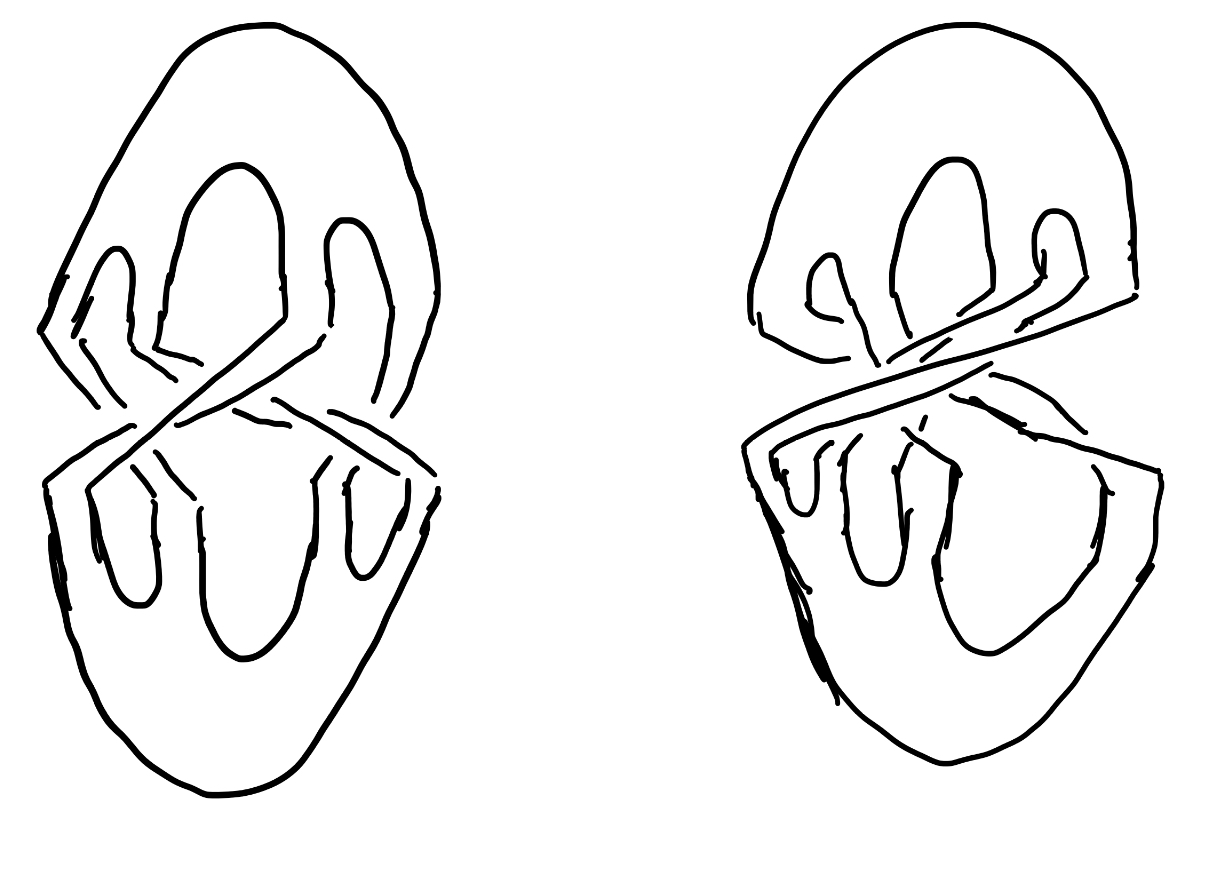
\includegraphics[scale = 0.1]{pictures_eskiz/trees.jpeg}
%     \textcolor{red}{do as figure.} Picture of two elements of $\F_\Tau(H)$, second is $(\zeta, \omega)$. 
% \end{center}
    
% It is easy to see, that 
% \begin{enumerate}
%     \item $\F_\Tau(1)$ is the Thomspon's group $F$
%     \item $\F_\Tau(\ZZ/n)$ is the Thomspon's group $T$
%     \item $\F_\Tau(S_n)$ is the Thomspon's group $V$
% \end{enumerate}
% Using the machinery described in \cite{Witzel_2019} \textcolor{red}{check reference} we can also prove the following statement.
% \begin{lemma}
%     The 7 final Thompson's groups are of type $F_\infty$.
% \end{lemma}
% The second point of view that we might take is topological. As in the general theory of Thompson's groups, we can prove that all the 7 final Thomspon's groups have faithful \textcolor{red}{check if it is the correct term} representations in $\text{Homeo}(\textsf{cantor set})$. 

% Naturally, we need to build this representation only for the largest of these final groups $\F_\Tau(H_*)$. 

% Denote as $\CC$ the Cantor set viewed as a subspace of $\RR$. Define 
% $$\cantor : 1/\Tau \to \text{compact subsets of } [0, 1]$$ so that $\cantor(t)$ is the subdivision of $[0,1]$ set corresponding to $t$ (as in the standard definition of the Cantor set). That is, $\cantor(*) = [0,1]$ and for all $t \in \Tau$ one has  $\CC = \bigcap_{t \in \Tau} \cantor(t)$. For any tree $t$ denote by $J_t$ the inclusion $\CC \to \cantor(t)$. Also, for a tree $t \in \Tau$ denote $|t| := \text{number of leaves in } t$.

% Now the following is a simple observation.  
% \begin{lemma}
%     Consider the subgroup of $\text{Homeo}(\CC)$ generated by elements $f$ of the following kind: for any two $t, t' \in 1/\Tau$ with equal number of leaves $f$ is induced from any piecewise linear (maybe with orientation reversal) homeomorphism $\cantor(t) \to \cantor(t')$. Then this subgroup is isomorphic to $\F_\Tau(H).$
% \end{lemma}
% \begin{center}
%     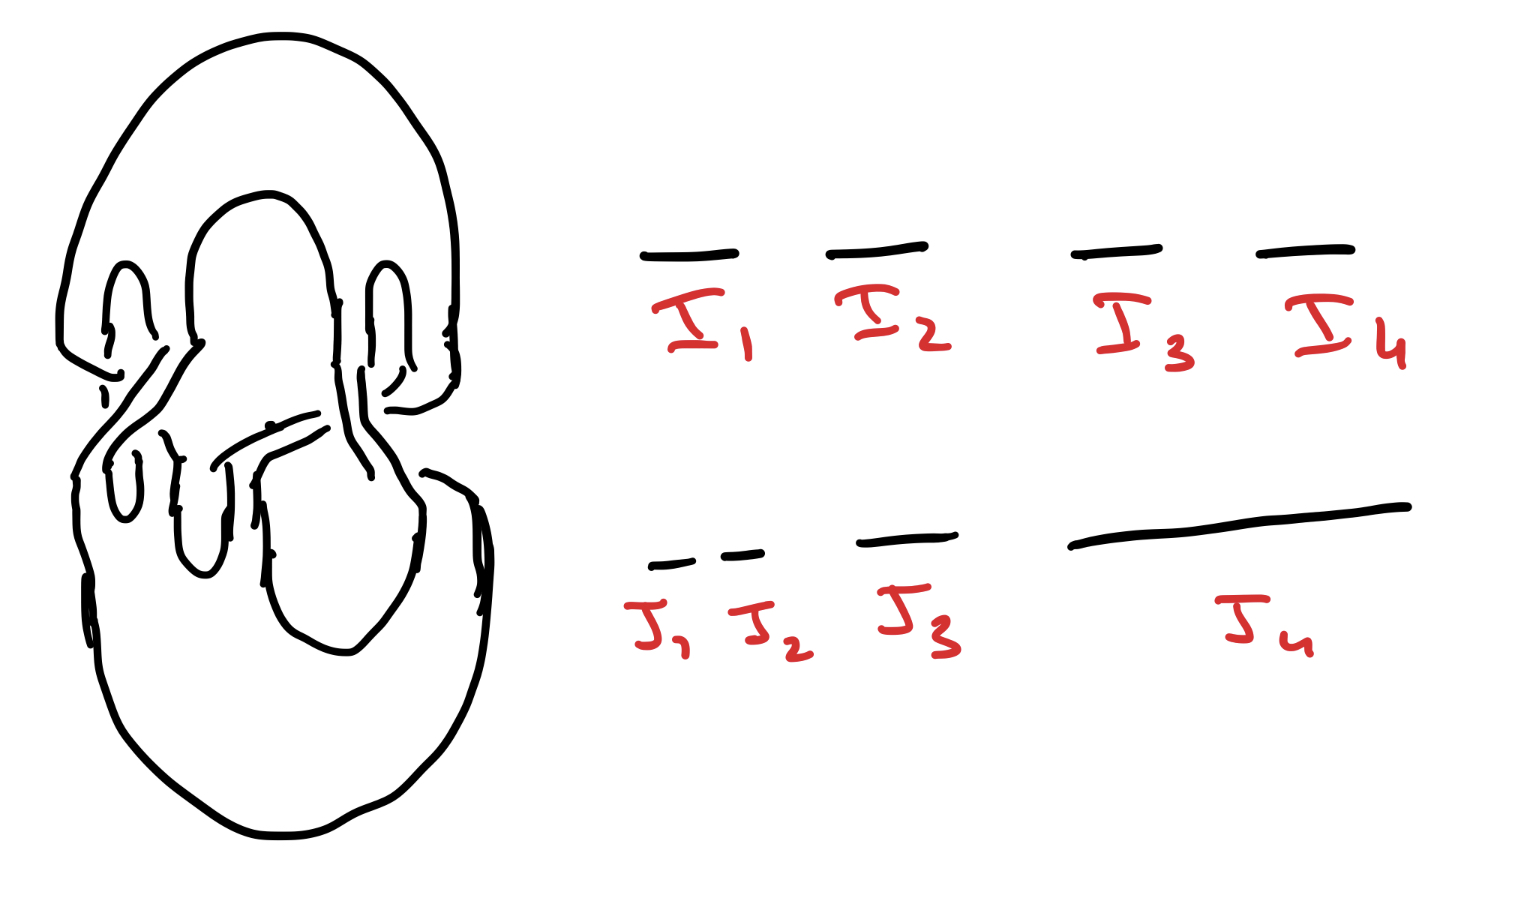
\includegraphics[scale = 0.1]{pictures_eskiz/cantors.jpeg}
%     \textcolor{red}{do as figure.} 
% \end{center}

% For the sake of the story, we compute their abelianizations. 
% \begin{lemma}
%     The abelianizations of the 7 final generalized Thompson's groups are the following: 
%     \begin{enumerate}
%         \item For $\F_\Tau(1)$ it is $\ZZ^2$
%         \item For other it is \textcolor{red}{is it?} 0. 
%     \end{enumerate}
% \end{lemma}


\section{Closed under subgroups}
In this section we prove the following result: the class of all generalized Thompson's groups (without a fixed base category) is closed under subgroups. That is, we prove the following theorem.
\begin{theorem}\label{Theorem-B}
    Let $H \leq \F_\cc(G)$ be a subgroup of a generalized Thompson's group. Then there exist $\dd \in \GOCat_\ast, N \in \GOCrossed(\dd)$ such that $H = \F_\dd(N)$. Also, the construction of $\dd$ and $N$ is functorial. 
\end{theorem}


For the proof we use a reformulation of the Galois correspondence principle in the groupoid language (see \cite{may_concise_1999}).

\begin{definition}
    Let $\ee, \bb$ be two small groupoids. A cover $p \colon \ee \to \bb$ is a functor such that \begin{enumerate}
        \item It is surjective on objects;
        \item It is bijective on the slice-categories $x/\ee$ for all $x \in \Obj(\ee)$. 
    \end{enumerate}
\end{definition}

As usual, all covers of a fixed groupoid $\bb$ form a category, which we denote $\Cov(\bb)$. In order to formulate the Galois correspondence, we need to introduce the category $\Subgroup G$ for a group $G$. Put
\begin{enumerate}
    \item Objects of $\Subgroup G$ to be the subgroups of $G$, 
    \item Morphisms from $H \leq G$ to $N \leq G$ to be the set $\{ g \in  G \; : \; g^{-1}Hg \subset N\}$ with the obvious composition law.
\end{enumerate}

\begin{theorem}[Galois correspondence theorem, ch. 3 in \cite{may_concise_1999}]
    Let $\Gamma$ be a small connected groupoid with a fixed object. There is a natural in $\Gamma$ equivalence of categories: 
    $$\Tilde{\Eps} : \Subgroup G \longleftrightarrow \Cov(\Gamma) : \pi_1$$
\end{theorem}


\subsection*{Proof of Theorem \ref{Theorem-B}}
Let $H \leq \F_\cc(G)$ be a subgroup. Then by the Galois correspondence we obtain a group covering $E \to \Loc \cc G$. Consider the following pushout diagram. 

% https://q.uiver.app/#q=WzAsNixbMCwyLCJcXG1hdGhjYWx7Q30iXSxbMiwyLCJcXG1hdGhjYWx7Q31HIl0sWzQsMiwiXFx0ZXh0e0xvY31cXCxcXG1hdGhjYWx7Q31HIl0sWzQsMCwiRSJdLFsyLDAsIlgiXSxbMCwwLCJXIl0sWzMsMiwiXFx0ZXh0e2NvdmVyfSJdLFsxLDJdLFs0LDFdLFs0LDNdLFs0LDIsIiIsMCx7InN0eWxlIjp7Im5hbWUiOiJjb3JuZXIifX1dLFswLDFdLFs1LDBdLFs1LDRdLFs1LDEsIiIsMCx7InN0eWxlIjp7Im5hbWUiOiJjb3JuZXIifX1dXQ==
\[\begin{tikzcd}
	\mathcal{Q} && X && E \\
	\\
	{\mathcal{C}} && {\mathcal{C}G} && {\text{Loc}\,\mathcal{C}G}
	\arrow[from=1-1, to=1-3]
	\arrow[from=1-1, to=3-1]
	\arrow["\lrcorner"{anchor=center, pos=0.125}, draw=none, from=1-1, to=3-3]
	\arrow[from=1-3, to=1-5]
	\arrow[from=1-3, to=3-3]
	\arrow["\lrcorner"{anchor=center, pos=0.125}, draw=none, from=1-3, to=3-5]
	\arrow["{\text{cover}}", from=1-5, to=3-5]
	\arrow[from=3-1, to=3-3]
	\arrow[from=3-3, to=3-5]
\end{tikzcd}\]

We will utilize the following two technical statements that we prove below. 

\begin{lemma}\label{technical1}
    Let $\cc$ be a connected Ore category, let $p \colon E \to \Loc \cc$ be a groupoid covering. Then $\cc \times_{\Loc \cc} E$ is an Ore category. Also, the structural map~ $\pi_E \colon \cc \times_{\Loc \cc} E \to E$ induces an equivalence of categories: 
    $$\Loc(\cc \times_{\Loc \cc} E ) \to E.$$
\end{lemma}

\begin{lemma}\label{technical2}
    In the diagram above
    \begin{enumerate}
        \item The category $\qq$ is a connected gaunt Ore category,
        \item The functor $\qq \to X$ is an inclusion of a $\GOCat$ category into its crossed group category. 
    \end{enumerate}
\end{lemma}

Using lemma \ref{technical2} we conclude that $X = \qq N_*$ for some crossed $\qq$-group $N_*$. Using lemma \ref{technical1} we see that $E = \Loc \qq N_*$. Hence, $H = \pi_1(\Loc \qq N_*) =: \F_\qq(N)$. By the fact that the construction is a pushout, $\qq$ and $N$ are functorial. 

% \begin{lemma}
    
% \end{lemma}




% \section{The Witzel's results}
% Here we \textcolor{blue}{talk about, investigate} what follows from the Witzel's paper \cite{Witzel_2019}. Note that in the context of Witzel the crossed group category $\cc G$ is a Zappa-Szép product of $\cc$ and the disconnected groupoid $\bigsqcup_{t \in \cc} G_t$.


% \textcolor{red}{formulate them in our context}\ \\ 
% \textcolor{red}{prove that 7 are f infty}

% \section{Examples}
% All the existing examples of thompson's groups. Also: other categories, fractal sets.




\section{Proofs}

\begin{proof}[Proof of the lemma \ref{Normal-form}]
    By lemma \ref{word-problem-loc} there exist $r_1, r_2 \in \cc G$ so that $t_1g r_1 = r_2 = t_2r_1$. By the definition of $\cc G$ decompose $r_1 = T_1 h_1, r_2 = T_2h_2$ with $T_i \in \Arr(\cc), h_i \in G_\ast$. So we get: 
    $$t_1 g T_1h_1 = T_2h_2 = t_2T_1h_1.$$
    From these equations it follows that $T_1^*(g) = 1$, by the injectivity we get that $g = 1$, $h_1 = h_2$. We deduce from above the equality $t_1T_1h_1 = t_2T_1 h_1$. Canceling from right we get that $t_1 = t_2$.
\end{proof}

\begin{proof}[Proof of the lemma \ref{CrossedOreLocalize}]
    
    \textbf{Right Cancellability}. For $a, b, c \in \cc$ let $(\alpha, g), (\gamma, r) : b \to c$ and $(\beta, h) : \alpha \to \beta$ be morphisms such that
    $(\alpha, g)\cdot(\beta, h) = (\gamma, r)\cdot(\beta, h)$. If one unfolds the definitions, this equality means that 
    $$(\alpha \circ g_* (\beta),\, \beta^*(g) \cdot h) = (\gamma \circ r_* (\beta),\, \beta^*(r) \cdot h).$$
    Now in the second coordinate by the injectiveness of $\beta^*$ one gets $g = r$ and then by the cancellability in $\cc$ one gets $\alpha = \gamma$. 

    \textbf{Left Cancellability}. Same argument, but one uses the fact that $g_*$ is a bijection. 

    \textbf{Common right multiples}. For two arrow $(\alpha, g), (\gamma, r) \in \Arr(\cc G_*)$, using \textsf{CRM} property for $\cc$ one gets two arrows $A, B \in \Arr(\cc)$ such that $\alpha A = \gamma B$. Put $\beta := (g^{-1})_*(A), \delta := (r^{-1})_*(B)$ and $h := (\beta^*(g))^{-1}, p := (\delta^*(r))^{-1}$. With these definitions one gets two following products which coincide by definition of $A, B$: 
    $$(\alpha, g)(\beta, h) = (\alpha \cdot g_*(\beta), \beta^*(g) \cdot h) = (\alpha A, 1_G),$$
    $$(\gamma, r) (\delta, p) = (\gamma \cdot r_*(\delta), \delta^*(r) \cdot p) = (\gamma B, 1).$$

Now for the necessity, putting $G = \{1\}$ we get that the condition (2) is necessary. 

% If presheaf action is not injective we have the following counter example. 

\end{proof}

\begin{proof}[Proof of the lemma \ref{technical1}]
    Let us denote $X := \cc \times_{\Loc \cc} E$. From general considerations, it follows that the category $X$ can be described as follows:
\begin{enumerate}
  \item Objects of $X$ are pairs $(c, e)$, where $c \in \cc, e \in E$, with the condition that $c = p(e)$.
  \item Morphisms in $X$, $(c_1, e_1) \to (c_2, e_2)$, are pairs of morphisms $f_1 \in \cc(c_1, c_2), f_2 \in E(e_1,e_2)$ such that $p(f_2) = \loc(f_1)$. 
\end{enumerate}

\textbf{Right cancellability}. 
Take morphisms $p = (p_1, p_2), q = (q_1, q_2), r = (r_1, r_2)$ such that $pq = rq$. Then,
$$p_1q_1 = r_1q_1 \Longrightarrow p_1 = r_1 \quad (\text{O1 for } \cc),$$
$$p_2q_2 = r_2q_2 \Longrightarrow p_2 = r_2 \quad (E \text{ is a groupoid}).$$

\textbf{Left cancellability}. A similar argument applies.

\textbf{Right divisors}.

Suppose that two morphisms $p = (p_1, p_2)$ and $q = (q_1, q_2)$ have the same domain. Then by axiom O2, there exist morphisms $r_1, s_1$ such that $p_1r_1 = q_1s_1$. 


% https://q.uiver.app/#q=WzAsOCxbMCwzLCJjXzEiXSxbMiwzLCJjXzMiXSxbMSwyLCJjXzIiXSxbMywyLCJjXzQiXSxbMCwxLCJlXzEiXSxbMSwwLCJlXzIiXSxbMiwxLCJlXzMiXSxbMywwLCJlXzQiXSxbMCwyLCJwXzEiXSxbMCwxLCJxXzEiLDJdLFsyLDMsIlxcZXhpc3RcXDsgcl8xIiwwLHsibGFiZWxfcG9zaXRpb24iOjMwLCJzdHlsZSI6eyJib2R5Ijp7Im5hbWUiOiJkYXNoZWQifX19XSxbMSwzLCJcXGV4aXN0IFxcOyBzXzEiLDIseyJzdHlsZSI6eyJib2R5Ijp7Im5hbWUiOiJkYXNoZWQifX19XSxbNCwwLCIiLDIseyJzdHlsZSI6eyJ0YWlsIjp7Im5hbWUiOiJtYXBzIHRvIn0sImJvZHkiOnsibmFtZSI6ImRvdHRlZCJ9fX1dLFs1LDIsIiIsMix7InN0eWxlIjp7InRhaWwiOnsibmFtZSI6Im1hcHMgdG8ifSwiYm9keSI6eyJuYW1lIjoiZG90dGVkIn19fV0sWzYsMSwiIiwyLHsic3R5bGUiOnsidGFpbCI6eyJuYW1lIjoibWFwcyB0byJ9LCJib2R5Ijp7Im5hbWUiOiJkb3R0ZWQifX19XSxbNywzLCIiLDIseyJzdHlsZSI6eyJ0YWlsIjp7Im5hbWUiOiJtYXBzIHRvIn0sImJvZHkiOnsibmFtZSI6ImRvdHRlZCJ9fX1dLFs0LDUsInBfMiIsMV0sWzQsNiwicV8yIiwxLHsibGFiZWxfcG9zaXRpb24iOjcwfV0sWzUsNywicl8yIiwyLHsic3R5bGUiOnsiYm9keSI6eyJuYW1lIjoiZGFzaGVkIn19fV0sWzYsNywic18yIiwyLHsic3R5bGUiOnsiYm9keSI6eyJuYW1lIjoiZGFzaGVkIn19fV1d
\[\begin{tikzcd}
  & {e_2} && {e_4} \\
  {e_1} && {e_3} \\
  & {c_2} && {c_4} \\
  {c_1} && {c_3}
  \arrow["{r_2}"', dashed, from=1-2, to=1-4]
  \arrow[dotted, maps to, from=1-2, to=3-2]
  \arrow[dotted, maps to, from=1-4, to=3-4]
  \arrow["{p_2}"{description}, from=2-1, to=1-2]
  \arrow["{q_2}"{description, pos=0.7}, from=2-1, to=2-3]
  \arrow[dotted, maps to, from=2-1, to=4-1]
  \arrow["{s_2}"', dashed, from=2-3, to=1-4]
  \arrow[dotted, maps to, from=2-3, to=4-3]
  \arrow["{\exists\; r_1}"{pos=0.3}, dashed, from=3-2, to=3-4]
  \arrow["{p_1}", from=4-1, to=3-2]
  \arrow["{q_1}"', from=4-1, to=4-3]
  \arrow["{\exists \; s_1}"', dashed, from=4-3, to=3-4]
\end{tikzcd}\]

Let $P_o$ be the bijection induced by $p$ on the sets $e_1/E$ and $c_1/\Loc \cc$. Define $r_2 := p_2^{-1}P_o^{-1}(p_1r_1)$ and $s_2 := q_2^{-1}P_o^{-1}(q_1s_1)$. 

\textbf{Equivalence of categories $\Loc X$ and $E$}.  
The map $\loc^* \colon X \to E$ induces a functor of groupoids $\varphi \colon \Loc X \to E$ by the universal property. We want to prove that this is an equivalence of categories.  

It is clearly surjective on objects: it maps the pair $(c, e)$ to the object $e \in E$, and from the definition of a covering, we obtain surjectivity (in particular, essential surjectivity). 

% https://q.uiver.app/#q=WzAsMTAsWzAsMywiY18xIl0sWzIsMiwiY18zIl0sWzIsNCwiY180Il0sWzQsMywiY18yIl0sWzEsMSwiZV8xIl0sWzMsMCwiZV8zIl0sWzMsMiwiZV80Il0sWzUsMSwiZV8yIl0sWzIsMywiY18wIl0sWzMsMSwiZV8wIl0sWzAsMV0sWzAsMl0sWzMsMl0sWzMsMV0sWzQsMCwiIiwwLHsic3R5bGUiOnsidGFpbCI6eyJuYW1lIjoibWFwcyB0byJ9LCJib2R5Ijp7Im5hbWUiOiJkYXNoZWQifX19XSxbNSwxLCIiLDAseyJzdHlsZSI6eyJ0YWlsIjp7Im5hbWUiOiJtYXBzIHRvIn0sImJvZHkiOnsibmFtZSI6ImRhc2hlZCJ9fX1dLFs2LDIsIiIsMCx7InN0eWxlIjp7InRhaWwiOnsibmFtZSI6Im1hcHMgdG8ifSwiYm9keSI6eyJuYW1lIjoiZGFzaGVkIn19fV0sWzcsMywiIiwwLHsic3R5bGUiOnsidGFpbCI6eyJuYW1lIjoibWFwcyB0byJ9LCJib2R5Ijp7Im5hbWUiOiJkYXNoZWQifX19XSxbMSw4XSxbMiw4XSxbOSw4LCIiLDIseyJzdHlsZSI6eyJ0YWlsIjp7Im5hbWUiOiJtYXBzIHRvIn0sImJvZHkiOnsibmFtZSI6ImRhc2hlZCJ9fX1dLFs0LDVdLFs0LDZdLFs3LDVdLFs3LDZdLFs1LDldLFs2LDldXQ==
\[\begin{tikzcd}
	&&& {e_3} \\
	& {e_1} && {e_0} && {e_2} \\
	&& {c_3} & {e_4} \\
	{c_1} && {c_0} && {c_2} \\
	&& {c_4}
	\arrow[from=1-4, to=2-4]
	\arrow[dashed, maps to, from=1-4, to=3-3]
	\arrow[from=2-2, to=1-4]
	\arrow[from=2-2, to=3-4]
	\arrow[dashed, maps to, from=2-2, to=4-1]
	\arrow[dashed, maps to, from=2-4, to=4-3]
	\arrow[from=2-6, to=1-4]
	\arrow[from=2-6, to=3-4]
	\arrow[dashed, maps to, from=2-6, to=4-5]
	\arrow[from=3-3, to=4-3]
	\arrow[from=3-4, to=2-4]
	\arrow[dashed, maps to, from=3-4, to=5-3]
	\arrow[from=4-1, to=3-3]
	\arrow[from=4-1, to=5-3]
	\arrow[from=4-5, to=3-3]
	\arrow[from=4-5, to=5-3]
	\arrow[from=5-3, to=4-3]
\end{tikzcd}\]
\end{proof}






\begin{proof}[Proof of the lemma \ref{technical2}]
    First, note that the category $\qq$ can also be presented as the pullback $\cc \to \Loc(\cc \; G) \leftarrow E$. This follows from a well-known categorical result (also known as the pasting lemma), that in a commutative diagram as below, where the right square is a pullback, the left square is a pullback if and only if the outer rectangle is a pullback.
    \[\begin{tikzcd}
	\bullet & \bullet & \bullet \\
	\bullet & \bullet & \bullet
	\arrow[from=1-1, to=1-2]
	\arrow[from=1-1, to=2-1]
	\arrow[from=1-2, to=1-3]
	\arrow[from=1-2, to=2-2]
	\arrow["\lrcorner"{anchor=center, pos=0.125}, draw=none, from=1-2, to=2-3]
	\arrow[from=1-3, to=2-3]
	\arrow[from=2-1, to=2-2]
	\arrow[from=2-2, to=2-3]
\end{tikzcd}\]


Let us denote by $p \colon E \to \Loc \; \cc$ the covering map of interest. Then we obtain that
\begin{enumerate}
    \item Objects of $\qq$ are pairs $(c, e)$, where $c \in \cc, e \in E$ such that $p(e) = c$. 
    \item Morphisms in $\qq$ between $(c_1, e_1)$ and $(c_2, e_2)$ are pairs $(f \colon c_1 \to c_2, g \colon e_1 \to e_2)$ such that $p(g) = \loc(f)$. 
\end{enumerate}
From this description it immediately follows that the category $\qq$ is skeletal. Any isomorphism $f = (f_\cc, f_E) \colon (c, e) \to (c, e)$ must satisfy the following properties: $f_\cc = \id_c$, since $\cc$ is skeletal, and $p(f_E) = \id_c$ by definition. By the definition of a covering, $f_E$ must also be equal to $\id_e$. 

We will prove that $X$ is the category of a crossed group over $\qq$ using Lemma \ref{detectionlemma}: we need to prove that any morphism in $X$ can be uniquely factored as a composition of a morphism from $\qq$ and an automorphism.

% https://q.uiver.app/#q=WzAsNixbMCwwLCJlXzEiXSxbMiwwLCJlXzIiXSxbNCwwLCJlXzIiXSxbMCwyLCJjXzEiXSxbMiwyLCJjXzIiXSxbNCwyLCJjXzIiXSxbMyw0LCJcXGluIFxcbWF0aGNhbHtDfSIsMl0sWzQsNSwiXFxpbiBHX3tjXzJ9IiwyXSxbMCwzLCIiLDIseyJzdHlsZSI6eyJ0YWlsIjp7Im5hbWUiOiJtYXBzIHRvIn0sImJvZHkiOnsibmFtZSI6ImRvdHRlZCJ9fX1dLFsxLDQsIiIsMix7InN0eWxlIjp7InRhaWwiOnsibmFtZSI6Im1hcHMgdG8ifSwiYm9keSI6eyJuYW1lIjoiZG90dGVkIn19fV0sWzIsNSwiIiwwLHsic3R5bGUiOnsidGFpbCI6eyJuYW1lIjoibWFwcyB0byJ9LCJib2R5Ijp7Im5hbWUiOiJkb3R0ZWQifX19XSxbMCwxLCJcXGV4aXN0cyIsMSx7InN0eWxlIjp7ImJvZHkiOnsibmFtZSI6ImRhc2hlZCJ9fX1dLFswLDIsIlxcZXhpc3RzIiwwLHsibGFiZWxfcG9zaXRpb24iOjQwLCJjdXJ2ZSI6LTMsInN0eWxlIjp7ImJvZHkiOnsibmFtZSI6ImRhc2hlZCJ9fX1dXQ==
\[\begin{tikzcd}
	{e_1} && {e_2} && {e_2} \\
	\\
	{c_1} && {c_2} && {c_2}
	\arrow["\exists"{description}, dashed, from=1-1, to=1-3]
	\arrow["\exists"{pos=0.4}, curve={height=-18pt}, dashed, from=1-1, to=1-5]
	\arrow[dotted, maps to, from=1-1, to=3-1]
	\arrow[dotted, maps to, from=1-3, to=3-3]
	\arrow[dotted, maps to, from=1-5, to=3-5]
	\arrow["{\in \mathcal{C}}"', from=3-1, to=3-3]
	\arrow["{\in G_{c_2}}"', from=3-3, to=3-5]
\end{tikzcd}\]

Coming up with such a factorization is not difficult: a morphism $(c_1, e_1) \to (c_2, e_2)$ in the category $X$ is a pair of morphisms $f \colon c_1 \to c_2$ and $g \colon e_1 \to e_2$. The first of them decomposes (uniquely) as a composition $f = f_\cc f_{G_{c_2}}$, and we consider the liftings of these morphisms under the covering in the slice category $e_1/E$, which gives the desired factorization. It is unique due to the uniqueness of the decomposition of $f$.


\end{proof}


\printbibliography


% \bibliography{reference}
% \bibliographystyle{alphaurl}

\end{document}
